%------------------------------------------------
%	PACKAGES AND THEMES
%------------------------------------------------
\documentclass{beamer}
\mode<presentation> {
    \usetheme[block=fill, sectionpage=none]{metropolis}
    % \usecolortheme{metropolis-highcontrast}
    % \usefonttheme[onlymath]{serif}
    \setbeamercolor{normal text}{bg=white}
}
% \setbeameroption{show notes on second screen=right}
% \setbeamertemplate{note page}{\pagecolor{yellow!5}\insertnote}
% \setsansfont{Ubuntu}
% \setmonofont{Ubuntu Mono}
% \setsansfont[BoldFont={Fira Sans SemiBold}]{Fira Sans Book}

\usepackage[export]{adjustbox}
\usepackage{amsmath}
\usepackage{amsthm}
\usepackage{amssymb}
\usepackage{amsfonts}
\usepackage{bbding}
\usepackage{cancel}
\usepackage{caption}
\usepackage{centernot}
\usepackage{comment}
% \usepackage{enumerate}
\usepackage[shortlabels]{enumitem}
\usepackage{epsfig}
\usepackage{epstopdf}
\usepackage[letterpaper, top=1.0in, bottom=1.0in, left=1.0in, right=1.0in]{geometry}
\usepackage{graphics}
\usepackage{graphicx}
\graphicspath{{figures/}}
\usepackage{IEEEtrantools}
\usepackage{ifpdf}
\usepackage{lastpage}
\usepackage{leftidx}
\usepackage{mathrsfs}
\usepackage{mathtools}
\usepackage{multicol}
\usepackage{multirow}
\usepackage[square, numbers, comma, sort&compress]{natbib}
\usepackage{nicefrac}
\usepackage{nicematrix}
\usepackage{outlines}
\usepackage{paralist}
\usepackage{pgfplots}
% \usepackage{pslatex}
\usepackage{ragged2e}
\usepackage{rotating}
\usepackage{stmaryrd}
\usepackage{subcaption}
\usepackage{tikz}
\usepackage{tkz-euclide}
\usepackage{ctable}
\usetikzlibrary{matrix, arrows}
\usepackage{tabularx}
\usepackage{todonotes}
\usepackage{ulem}
\usepackage{units}
\usepackage{url}
\usepackage{wrapfig}
\usepackage{xcolor}


% \hypersetup{
%     bookmarks=true,         % show bookmarks bar?
%     unicode=false,          % non-Latin characters in Acrobat’s bookmarks
%     pdftoolbar=true,        % show Acrobat’s toolbar?
%     pdfmenubar=true,        % show Acrobat’s menu?
%     pdffitwindow=false,     % window fit to page when opened
%     pdfstartview={FitH},    % fits the width of the page to the window
%     pdftitle={My title},    % title
%     pdfauthor={Author},     % author
%     pdfsubject={Subject},   % subject of the document
%     pdfcreator={Creator},   % creator of the document
%     pdfproducer={Producer}, % producer of the document
%     pdfkeywords={keyword1, key2, key3}, % list of keywords
%     pdfnewwindow=true,      % links in new PDF window
%     colorlinks=false,       % false: boxed links; true: colored links
%     linkcolor=blue,          % color of internal links (change box color with linkbordercolor)
%     linkbordercolor=orange,
%     citecolor=green,        % color of links to bibliography
%     citebordercolor=blue,
%     filecolor=magenta,      % color of file links
%     urlcolor=cyan,           % color of external links
%     urlbordercolor=blue
% }

\makeatletter
\newcommand{\rmnum}[1]{\romannumeral #1}
\newcommand{\Rmnum}[1]{\expandafter\@slowromancap\romannumeral #1@}
\makeatother

\newcommand{\bmat}[1]{\begin{bmatrix}#1\end{bmatrix}}
\newcommand{\ubar}[1]{\text{\b{$#1$}}}
\newcommand{\norm}[2]{\left\|{#1}\right\|_{{}_{#2}}}
\newcommand{\abs}[1]{\left|{#1}\right|}
\newcommand{\mbf}[1]{\mathbf{#1}}
\newcommand{\mc}[1]{\mathcal{#1}}
\newcommand{\dd}{\operatorname{d}\!}
\newcommand{\muc}[2]{\multicolumn{#1}{c}{#2}}
\newcommand*\Eval[3]{\left.#1\right\rvert_{#2}^{#3}}
\newcommand{\inner}[1]{\left\langle#1\right\rangle}
\newcommand{\pd}[2]{\frac{\partial #1}{\partial #2}}
\newcommand{\pdd}[2]{\frac{\partial^2 #1}{\partial #2^2}}
\newcommand{\el}[2]{\frac{\dd}{\dd t}\pd{\mc{L}}{\dot{#1}} - \pd{\mc{L}}{#1} = #2}
\newcommand{\elk}[2]{\frac{\dd}{\dd t}\pd{\mc{L}}{\dot{#1}_k} - \pd{\mc{L}}{#1_k} = #2_k}
\newcommand{\vectornorm}[1]{\left|\left|#1\right|\right|}
\newcommand{\dom}[1]{\textrm{dom}\;#1}
\newcommand\blfootnote[1]{%
  \begingroup
  \renewcommand\thefootnote{}\footnote{#1}%
  \addtocounter{footnote}{-1}%
  \endgroup
}
\newcommand{\bx}{{\bf x}}
\newcommand{\bu}{{\bf u}}

\newtheorem{defn}{Definition}
\newtheorem{thm}{Theorem}[section]
\newtheorem{lem}[thm]{Lemma}
\newtheorem{prop}{Proposition}[section]
\newtheorem{rem}{Remark}

\DeclareMathOperator{\Tr}{tr}
\newcommand\xdownarrow[1][2ex]{%
   \mathrel{\rotatebox{90}{$\xleftarrow{\rule{#1}{0pt}}$}}
}
\DeclareMathOperator{\End}{End}
\DeclareMathOperator{\Hom}{Hom}
\DeclareMathOperator{\id}{id}
\DeclareMathOperator{\vers}{vers}
\DeclareMathOperator{\trans}{Trans}
\DeclareMathOperator{\rot}{Rot}
\DeclareMathOperator{\rank}{rank}


\makeatletter
\newcommand{\xMapsto}[2][]{\ext@arrow 0599{\Mapstofill@}{#1}{#2}}
\def\Mapstofill@{\arrowfill@{\Mapstochar\Relbar}\Relbar\Rightarrow}
\newcommand{\xMapsfrom}[2][]{\ext@arrow 0599{\Mapsfromfill@}{#1}{#2}}
\makeatother


% \AtBeginSection[]
% {
%     \begin{frame}[plain, noframenumbering]
%         \frametitle{Outline}
%         \tableofcontents[currentsection]
%         % \tableofcontents[currentsection, currentsubsection]
%     \end{frame}
% }

%------------------------------------------------
%   TITLE PAGE
%------------------------------------------------
\title[] {
    Nonlinear Systems
}
\subtitle[]{
    Morse Theory and Lyapunov Stability on Manifolds
}
\author[Aykut C. Satici]{
    Aykut C. Satici \\
    $\,$ \\
}
\institute[BSU] {
    Boise State University \\
    % \medskip
    Mechanical and Biomedical Engineering \\%
    Electrical and Computer Engineering \\%
    % \medskip
    % Doctoral Comprehensive Examination
}
\date{March 12, 2021}

\begin{document}

\begin{frame}[plain, noframenumbering]
\titlepage
\end{frame}

%------------------------------------------------
%	PRESENTATION SLIDES
%------------------------------------------------
\begin{frame}[plain, noframenumbering]
    \frametitle{Outline}
    \tableofcontents
    % \tableofcontents[hideallsubsections]
\end{frame}

\begin{frame}
    \frametitle{Lyapunov stability theory}

    

    \begin{itemize}
        \item Introduced by Alexandr Mikhailovich Lyapunov.
        \item \textit{The general problem of the stability of motion}, 1892.
        \item Doctoral thesis in Kharkov Mathematical Society.
        \item The most general theory for analyzing stability of (at least)
        ordinary differential equations.
    \end{itemize}

\end{frame}
\section{Notations and Definitions}

\begin{frame}[standout, plain, noframenumbering]
    Notations and Definitions

    % \medskip

    % \footnotesize
    % Sam Greydanus \quad Misko Dzamba \quad Jason Yosinski
\end{frame}


\begingroup
\small

\begin{frame}
    \frametitle{Manifolds and Vector Fields}

    \begin{itemize}
        \item $\mc{M}$ (state-space) denotes a manifold of finite dimension $n$.
        \item $f \in \mathfrak{X}(M)$ is a continuous vector field on $\mc{M}$.
        \item We assume that there exists a unique right maximally defined
        integral curve of $f$ starting at $x$.
        \item We also assume that this integral curve is defined on $[0,
        \infty]$.
        \[
            \varphi: [0, \infty] \times \mc{M} \rightarrow \mc{M}
        \]
        with 
        \begin{align*}
            \varphi(0, x) &= x, \\
            \varphi(t_1, \varphi(t_2,x)) &= \varphi(t_1+t_2, x).
        \end{align*}
        \item The semiflow $\varphi$ is the evolution function.
    \end{itemize}
\end{frame}


\begin{frame}
    \frametitle{Invariant and Stable Sets}

    \begin{definition}
        $\Omega \subseteq \mc{M}$ is called an \textsc{invariant set} if for all
        $x \in \Omega$ and $t \in \mathbb{R}_{\geq 0}$, $\varphi(t,x) \in
        \Omega$. If $\Omega = \{p\}$ is a singleton, then $\Omega$ is called and
        \textsc{equilibrium point} of the dynamical system $(\mc{M}, \varphi)$.
    \end{definition}

    \begin{definition}
        $\Omega \subseteq \mc{M}$ is \textsc{stable} if for \textit{every open
        neighborhood} $\mc{U} \subseteq \mc{M}$ of $\Omega$, \textit{there
        exists a neighborhood} $\mc{V} \subseteq \mc{M}$ of $\Omega$ such that 
        $\varphi(t, \mc{V}) \subseteq \mc{U}$ for all $t \geq 0$.

        An \textit{invariant set} $\Omega$ is asymptotically stable if

        \begin{itemize}
            \item $\Omega$ is stable,
            \item $\Omega$ is attractive, i.e., for all $x \in \Omega$, there
            exists an open neighborhood $\mc{N} \subseteq \mc{M}$ of $\Omega$
            such that for all $x \in \mc{N}$, $\varphi(t, x) \xrightarrow[]{t
            \rightarrow \infty} \Omega$.
        \end{itemize}
    \end{definition}
\end{frame}


\begin{frame}
    \frametitle{Domain (Region) of Attraction}

    \textit{The} domain of attraction is denoted by
    \[ \mc{A} = \{ x \in \mc{M}: \varphi(t,x) \rightarrow \Omega \text{ as } t
    \rightarrow \infty \}. \]

    $\Omega$ is said to be \textsc{globally} asymptotically stable if $\mc{N} =
    \mc{M}$.

    \begin{definition}
        The \textsc{Lie derivative} of $V: \mc{M} \rightarrow \mathbb{R}$ along
        $f \in \mathfrak{X}(\mc{M})$ is defined by 
        %
        \begin{align*}
            \mc{L}_fV: \mc{M} &\rightarrow \mathbb{R}, \\
            p &\mapsto \dd V_p (f(p)).
        \end{align*}
    \end{definition}
\end{frame}


\begin{frame}
    \frametitle{Lyapunov Function}

    \begin{definition}
        Let $\mc{K}$ be an invariant set of the dynamical system $(\mc{M},
        \varphi)$. A continuous function $V: \mc{A} \rightarrow \mathbb{R}_{\geq
        0}$ is a \textsc{Lyapunov function} if

        \begin{itemize}
            \item $V(x) > 0$ for all $x \in \mc{A} \backslash \mc{K}$,
            \item $V(x) = 0$ for all $x \in \mc{K}$,
            \item $V$ is proper, i.e., $V^{-1}(B)$ is compact for all compact
            subset $B \subseteq \mathbb{R}_{\geq 0}$,
            \item $V$ is strictly decreasing along orbits of $\varphi$, i.e.,
            \vspace{-1mm}
            \[ V \circ \varphi(t,x) < V(x), \] \vspace{-1mm} for all $t > 0$ and
            $x \in \mc{A} \backslash \mc{K}$.

            If $V$ is differentiable, this condition may be replaced by
            %
            \[ \mc{L}_fV(x) < 0. \]
        \end{itemize}
    \end{definition}
\end{frame}


\begin{frame}
    \frametitle{(Nondegenerate) Critical Points}

    \begin{definition}
        Let $V: \mc{M} \rightarrow \mathbb{R}$ be a smooth function. A
        \textsc{critical point}, $p \in \mc{M}$, of $V$ is a point where the
        differential \[ \dd V_p: T_p\mc{M} \rightarrow \mathbb{R} \] has rank
        zero, i.e., in any local coordinate system $\{x_i\}_{1}^n$, one has
        $\pd{V}{x_i}(p) = 0$ for all $i = 1, \ldots, n$.
    \end{definition}

    \begin{definition}
        A critical point $p$ is \textsc{nondegenerate} if the Hessian $H_p(V)$
        is a nondegenerate bilinear form, i.e., if any coordinate system, the
        Hessian matrix \[ \left( \frac{ \partial^2 V }{ \partial x_i \partial
        x_j } \right)_{1 \leq i,j \leq n} \] is nondegenerate.
    \end{definition}
\end{frame}


\begin{frame}
    \frametitle{Nondegenerate Critical Points}

    \begin{definition}
        The dimension of the subspace of $T_p\mc{M}$ on which $H_p(V)$ is
        negative definite is called the \textsc{Morse index} of $V$ at $p$,
        denoted by $\text{ind}(V, p)$.
    \end{definition}

    \begin{definition}
        A $C^2$ function $V: \mc{M} \rightarrow \mathbb{R}$ is a \textsc{Morse
        function} if all its critical points are nondegenerate.
    \end{definition}

    \begin{definition}
        The \textsc{(sub)-level sets} of a function $V: \mc{M} \rightarrow
        \mathbb{R}$ are
        \begin{align*}
            \mc{M}_a &= V^{-1}\left( (-\infty, a] \right), \\
            \mc{M}_{a,b} &= V^{-1}\left( [a, b] \right). \\
        \end{align*}
    \end{definition}
\end{frame}


\begin{frame}
    \frametitle{Topological Definitions}

    \begin{itemize}
        \item A top. space is an \textsc{$n$-cell} if it is homeomorphic to
        $\mathbb{R}^n$.
        \item A top. space $X$ is \textsc{contractible} if it is
        \textit{homotopy equivalent} to the one-point space.
        \item A subspace $A$ of $X$ is called a \textsc{deformation retract} of
        $X$ if there exists a continuous function $ h: [0,1] \times X
        \rightarrow X $ such that for all $x \in X$, $a \in A$, 
        \begin{align*}
            h(0,x) &= x, \\
            h(1,x) &\in A, \\
            h(1,a) &= a.
        \end{align*}
        \item The $k^{\text{th}}$ \textsc{Betti number} of $\mc{M}$, denoted by
        $b_k$ is the rank of the $k^{\text{th}}$ homology group $H^k(\mc{M})$.
        \item The \textsc{Euler characteristic} of $\mc{M}$ is defined by
        \[ \chi(\mc{M}) = \sum_{i=1}^k (-1)^k b_k. \]
    \end{itemize}
\end{frame}

% \begin{frame}
%     \frametitle{Angular Velocity: The Fixed Axis Case}

%     \begin{columns}
%         \begin{column}{0.5\textwidth}
%             \begin{align*}
%                 \omega &= \dot{\theta}k, \\
%                 v &= \omega \times r.
%             \end{align*}
%         \end{column}
%         \begin{column}{0.5\textwidth}
%             \begin{figure}[bth]
%                 \centering
%                 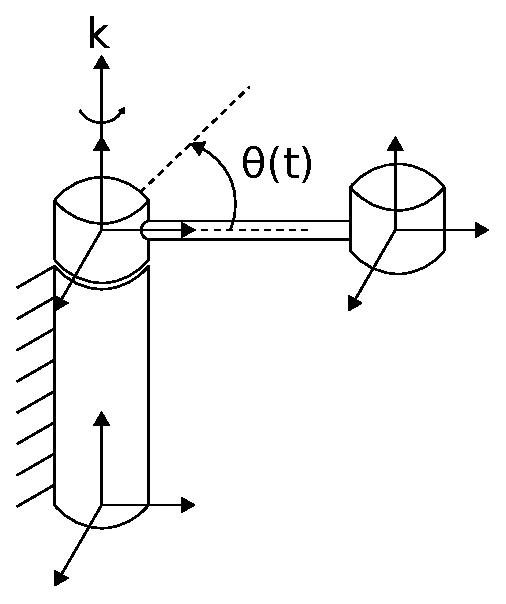
\includegraphics[width=0.5\textwidth]{figures/simple_rot.eps} 
%                 % \caption{\footnotesize Rotational motion of a one DoF manipulator.}
%             \end{figure}
%         \end{column}
%     \end{columns}

%     \begin{itemize}
%         \item In introductory dynamics courses, the computation of the linear
%         velocity $v$ is often the goal.
%         \item In our applications, we are interested in describing the motion of 
%         a moving frame:
%         \begin{itemize}
%             \footnotesize{
%             \item motion of the origin of the frame through space,
%             \item motion of the frame's axes.
%             }
%         \end{itemize}
%         \item For our purposes, the angular velocity will hold equal status with 
%         linear velocity.
%     \end{itemize}
% \end{frame}


% \begin{frame}
%     \frametitle{Angular Velocity: The Fixed Axis Case}
   

%     \begin{itemize}
%         \item The angular velocity is a property of the body-fixed coordinate
%         frame.
%         \item Angular velocity is \textit{not} a property of individual points.
%         \item Individual points may experience a \textbf{linear velocity} that 
%         is induced by an angular velocity, but it makes no sense to speak of a 
%         point itself rotating.
%         \item Thus, in equation~\eqref{eq:lin_vel_fixed}, $v$ corresponds to the 
%         linear velocity of a point, while $\omega$ corresponds to the angular 
%         velocity associated with a rotating coordinate frame.
%     \end{itemize}
% \end{frame}


% \begin{frame}
%     \frametitle{Angular Velocity: The Fixed Axis Case}

%     \begin{itemize}
%         \item In the fixed axis case, the problem of specifying angular 
%         displacements is really a planar problem
%         \begin{itemize}
%             \footnotesize{
%             \item each point traces out a circle,
%             \item every circle lies in a plane.
%             }
%         \end{itemize}
%         \item It is tempting to use $\dot{\theta}$ to represent the angular 
%         velocity.
%         \item However, this choice, does not generalize to the three-dimensional 
%         case.
%         \item We will develop a more general representation for angular velocities.
%         \item This will be analogous to our development of rotation matrices.
%         \item The key tool in this development is the skew-symmetric matrix.
%     \end{itemize}
% \end{frame}


\endgroup
\section{Morse-Lyapunov Functions}

\begin{frame}[standout, plain, noframenumbering]
    Morse-Lyapunov Functions

    % \medskip

    % \footnotesize
    % Sam Greydanus \quad Misko Dzamba \quad Jason Yosinski
\end{frame}

\begingroup
\small

\begin{frame}
    \frametitle{Isolated Critical Points}

    \begin{lemma}
        Suppose that $x_e$ is an equilibrium points of the dynamical system $(M,
        \varphi)$. If $V: \mc{M} \rightarrow \mathbb{R}$ is a differentiable
        Lyapunov function then $x_e$ is the only critical point of $V$.
    \end{lemma}

    \begin{proof}
        Suppose $V$ has another critical point, $x_c$, in the domain of
        attraction. By the definition of a Lyapunov function, we must have
        $\mc{L}_fV(x_c) = 0$. This contradicts the fact that if $x \neq x_e$,
        $\mc{L}_fV(x) < 0$.
    \end{proof}
\end{frame}


\begin{frame}
    \frametitle{Morse Lemma}

    \begin{theorem}[Morse Lemma]
        Let $p \in \mc{M}$ be a nondegenerate critical point of a smooth
        function $V: \mc{M} \rightarrow \mathbb{R}$. There exists a local
        coordinate system $\{x_i\}_1^n$ in a nbhd. $\mc{N} \subseteq \mc{M}$ of
        $p$ with $x_i(p) = 0$ for all $1 \leq i \leq n$ such that for $x \in
        \mc{N}$, \[ V(x) = V(p) - x_1^2 - \ldots - x_i^2 + x_{i+1}^2 + \ldots +
        x_n^2 \] where $i = \text{ind}(V,p)$.
    \end{theorem}

    \begin{corollary}
        Let $p \in \mc{M}$ be an equilibrium point of $(\mc{M}, \varphi)$ and
        $V: \mc{M} \rightarrow \mathbb{R}_{\geq 0}$ a Morse-Lyapunov function. 
        There exists a local coordinate system $\{x_i\}_1^n$ around $p$ such that 
        $V$ is locally the canonical quadratic Lyapunov function 
        \[ V(x) = \sum_{i=1}^n x_i^2 \] with $\text{ind}(V, p) = 0$.
    \end{corollary}
\end{frame}


\begin{frame}
    \frametitle{Level Sets of a Lyapunov Function}

    \begin{theorem}[Deformation Lemma]
        Let $V: \mc{M} \rightarrow \mathbb{R}$ be a smooth function and $a, b
        \in V(\mc{M})$ such that $a < b$. If $\mc{M}_{a,b}$ is compact and does
        not contain critical points of $V$ then $\mc{M}_a$ is diffeomorphic to
        $\mc{M}_b$. MOreover, $\mc{M}_a$ is a deformation retract of $\mc{M}_b$.
    \end{theorem}

    \begin{corollary}
        Let $\mc{M}$ be a smooth Riemannian manifold. If $\mc{M}$ contains a
        closed invariant asymptotically stable set, then for all $a, b \in
        V(\mc{M})$, $\mc{M}_a$ is diffeomorphic to $\mc{M}_b$ and $\mc{M}_a$ is
        a deformation retract of $\mc{M}_b$ where $V$ is a smooth Lyapunov
        function.
    \end{corollary}
\end{frame}


\endgroup
\section{Systems with Single Critical Points}

\begin{frame}[standout, plain, noframenumbering]
    Systems with Single Critical Points

    % \medskip

    % \footnotesize
    % Sam Greydanus \quad Misko Dzamba \quad Jason Yosinski
\end{frame}

\begingroup
\small

\begin{frame}
    \frametitle{Domain of Attraction -- Revisited}

    \begin{theorem}[Brown-Stallings Lemma]
        Let $\mc{M}$ be a paracompact manifold such that every compact subset is
        contained in an open set diffeomorphic to a Euclidean space. Then
        $\mc{M}$ itself is diffeomorphic to a Euclidean space.
    \end{theorem}

    \begin{corollary}
        Let $\mc{M}$ be a paracompact manifold. The domain of attraction of an
        asymptotically stable equilibrium point is diffeomorphic to a Euclidean
        space.
    \end{corollary}
\end{frame}

\begin{frame}
    \frametitle{Morse and Sontag Theorems}

    \begin{theorem}[Morse Theorem]
        Let $V: \mc{M} \rightarrow \mathbb{R}$ be a Morse function, $p$ a
        critical point such that $\text{ind}(V, p) = i$ and $c = V(p)$. If there
        exists $\varepsilon > 0$ such that $\mc{M}_{c-\varepsilon,
        c+\varepsilon}$ is compact and does not contain other critical points
        $p$, then $\mc{M}_{c-\varepsilon} \cup e_i$ is a deformation retract of
        $\mc{M}_{c+\varepsilon}$ where $e_i$ is an $i$-cell.
        % (in particular, $\mc{M}_{c+\varepsilon}$ has the homotopy type of
        % $\mc{M}_{c-\varepsilon}$ with an $i$-cell attached).
    \end{theorem}

    \begin{theorem}[Sontag Theorem]
        Let us consider the dynamical system $(\mc{M}, \varphi)$ with an
        equilibrium point $x_e \in \mc{M}$. Suppose that $x_e$ is asymptotically
        stable. Then the domain of attraction of $x_e$, given by 
        \[ \mc{A} = \left\{ x \in \mc{M}: \lim_{t \rightarrow \infty} \varphi(t,
        x) = x_e \right\}, \] is contractible.
    \end{theorem}
\end{frame}


\endgroup
\section{Systems with Multiple Critical Points}

\begin{frame}[standout, plain, noframenumbering]
    Systems with Multiple Critical Points

    % \medskip

    % \footnotesize
    % Sam Greydanus \quad Misko Dzamba \quad Jason Yosinski
\end{frame}

\begingroup
\small


\begin{frame}
    \frametitle{Morse Theorem -- (Third Version)}

    \begin{theorem}[Morse Theorem]
        If $V: \mc{M} \rightarrow \mathbb{R}$ is a Morse function such that 
        $\mc{M}_a$ is compact for each $a \in \mathbb{R}$ then $\mc{M}$ has the 
        homotopy type of a CW-complex with one $i$-cell for each critical point 
        of index $i$.
    \end{theorem}
    
    \begin{corollary}
        Suppose that the dynamical system $(\mc{M}, \varphi)$ has several
        equilibria $(x_1, \ldots, x_k)$. If there exists a Morse-Lyapunov
        function $V: \mc{M} \rightarrow \mathbb{R}_{\geq 0}$ then $\{x_1,
        \ldots, x_k\}$ is a retract of the domain of attraction.
    \end{corollary}

    \begin{prop}[Reeb Theorem]
        Suppose that $\mc{M}$ is compact without boundary. If $V: \mc{M}
        \rightarrow \mathbb{R}$ is a smooth function with only two critical
        points, then $\mc{M}$ is homeomorphic to the $n$-sphere $\mathbb{S}^n$.
    \end{prop}
\end{frame}

\begin{frame}
    \frametitle{Morse Inequalities}

    \begin{theorem}[Morse Inequalities]
        Let $m_k$ be the number of ciritcal points of a Morse function $V$ with
        index $k$. Then, we have

        \begin{align*}
            b_k &\leq m_k, \quad \forall k, \\
            \sum_{i=0}^j (-1)^{j-i}b_i &\leq \sum_{i=0}^j (-1)^{j-i}m_i \quad \forall j, \\
            \chi(\mc{M}) &= \sum_k (-1)^k b_k = \sum_k (-1)^k m_k.
        \end{align*}
    \end{theorem}

    The next corollary states a necesary condition for the existence of a
    Morse-Lyapunov function based on the Euler characteristic, which is a
    topological invariant.
\end{frame}


\begin{frame}
    \frametitle{Existence of Morse-Lyapunov Functions}

    \begin{corollary}
        Consider the dynamical system $(\mc{M}, \varphi)$ with several
        equilibria $(x_1, \ldots, x_k)$. If there exists a Morse-Lyapunov
        function $V: \mc{M} \rightarrow \mathbb{R}_{\geq 0}$ then $\chi(\mc{M})
        = k \geq b_0$.
    \end{corollary}

    \begin{proof}
        If there exists a Morse-Lyapunov function $V$, $(x_1, \ldots, x_k)$ are
        the only critical points with indices $0$. Then, by the Morse
        inequalities, $\chi(\mc{M}) = m_0 = k$ and $b_0 \leq m_0 = k$.
    \end{proof}

    \begin{rem}
        If $\chi(\mc{M}) \neq k$ then there is no Morse-Lyapunov function for
        the dynamical system.
    \end{rem}
\end{frame}

\endgroup
% \section{Linear Velocity of a Point Attached to a Moving Frame}

\begin{frame}[standout, plain, noframenumbering]
    Linear Velocity of a Point Attached to a Moving Frame

    % \medskip

    % \footnotesize
    % Sam Greydanus \quad Misko Dzamba \quad Jason Yosinski
\end{frame}

\begingroup
\small

\begin{frame}
    \frametitle{Linear Velocity of a Point Attached to a Moving Frame}

    \begin{itemize}
        \item Suppose the point $p$ is rigidly attached to $\Sigma_1$ and that 
        $\Sigma_1$ is rotating relative to the frame $\Sigma_0$.
        \[ p^0 = R_1^0(t)p^1. \]
        \item Differentiating this equation, we get 
        \[ \dot{p}^0 = \dot{R}_1^0 p^1 + \cancelto{0}{R_1^0 \dot{p}^1} =
        S\left( \omega^0 \right) R_1^0p^1 = S\left( \omega^0 \right) p^0 =
        \omega^0 \times p. \]
    \end{itemize}
\end{frame}


\begin{frame}
    \frametitle{Linear Velocity of a Point Attached to a Moving Frame}

    \begin{itemize}
        \item Now suppose that the motion of $\Sigma_1$ w.r.t. $\Sigma_0$ is
        more general and is given by \[ H_1^0(t) = \bmat{
            R(t) & o(t) \\ 0 & 1
        }. \]
        \item Hence we have $\qquad p^0 = Rp^1 + o$.
        \item Differentiating, we obtain,
        \[ \dot{p}^0 = \dot{R}p^1 + \dot{o} = S(\omega)Rp^1 + \dot{o} = \omega
        \times r + v, \] where $r = Rp^1$ is the vector from $o_1$ to $p$,
        expressed in $\Sigma_0$, and $v$ is the rate at which the origin $o_1$ 
        is moving.
        \item If the point $p$ is moving relative to $\Sigma_1$, then we must
        add to the term $v$ the term $R(t)\dot{p}^1$, which is the rate of
        change of the coordinates $p^1$, expressed in $\Sigma_0$.
    \end{itemize}
\end{frame}

\endgroup
% \section{Derivation of the Jacobian}

\begin{frame}[standout, plain, noframenumbering]
    Derivation of the Jacobian

    % \medskip

    % \footnotesize
    % Sam Greydanus \quad Misko Dzamba \quad Jason Yosinski
\end{frame}

\begingroup
\small


\begin{frame}
    \frametitle{Derivation of the Jacobian}

    \begin{itemize}
        \item Consider an $n$-link manipulator with joint variables $q_1, \ldots, q_n$. Let
        \[ T_n^0 = \bmat{R_n^0(q) & o_n^0(q) \\ 0 & 1} \] denote the
            transformation from the end effector frame $\Sigma_n$ to the base
            frame $\Sigma_0$.
        \item The objective of this section is to relate the linear and angular
        velocity of the end effector $\Sigma_n$ to the vector of joint
        velocities $\dot{q}(t)$. 
        \item Let \[ S\left( \omega_n^0 \right) = \dot{R}_n^0 \left( R_n^0 \right)^\top, \]
        denote the angular velocity vector $\omega_n^0$ of the end effector, and let
        \[ v_n^0 = \dot{o}_n^0, \] denote the linear velocity of the end effector.
    \end{itemize}
\end{frame}


\begin{frame}
    \frametitle{Derivation of the Jacobian}

    \begin{itemize}
        \item We seek expressions of the form
        \begin{align}
            v_n^0 &= J_v\dot{q} \label{eq:def_jac_v}, \\
            \omega_n^0 &= J_\omega\dot{q} \label{eq:def_jac_omega},
        \end{align}
        where $J_v, J_\omega \in \mathbb{R}^{3 \times n}$. Together, they can be
        written as 
        \[ \xi = J\dot{q}, \] in which $\xi$ and $J$ (\textbf{manipulator
        Jacobian} or \textbf{Jacobian}) are given by 
        \[ \xi = \bmat{v_n^0 \\ \omega_n^0} \quad \text{and} \quad J = \bmat{J_v \\ J_\omega}_{6 \times n}. \]
        \item This velocity vector $\xi$ is \textsc{not} the derivative of a
        position variable, since the angular velocity vector is not the
        derivative of any particular time-varying quantity.
    \end{itemize}
\end{frame}


\begin{frame}
    \frametitle{Angular Velocity}

    \begin{itemize}
        \item We can determine $\omega_{0,n}^0$ by expressing the angular velocity 
        contributed by each joint in $\Sigma_0$ and then summing these.
        \item If the joint $i$ is revolute, then the $i^{\textrm{th}}$ variable 
        $q_i$ equals $\theta_i$ and the axis of rotation is $z_{i-1}$.
        \item Recall $\omega_{i-1,i}^{i-1}$ represents the angular velocity of
        link $i$ that is imparted by the rotation of joint $i$, expressed
        relative to frame $\Sigma_{i-1}$. We have with $k = (0, 0, 1)$,
        \[ \omega_{i-1,i}^{i-1} = \dot{q}_i z_{i-1}^{i-1} = \dot{q}_ik. \]
        \item If the joint $i$ is prismatic, then the motion of $\Sigma_i$
        w.r.t. $\Sigma_1$ is a translation and \[ \omega_{i-1,i}^{i-1} = 0. \]
    \end{itemize}
\end{frame}

\begin{frame}
    \frametitle{Angular Velocity}

    \begin{itemize}
        \item Therefore, the overall angular velocity of the end effector
        $\omega_{0,n}^0$ is determined by 
        \begin{align*}
            \omega_{0,n}^0 &= \omega_{0,1}^0 + R_1^0\omega_{1,2}^1 + R_2^0\omega_{2,3}^2 + \cdots + R_n^0\omega_{n-1,n}^{n-1} \\ 
            &= \rho_1 \dot{q}_1k + \rho_2 \dot{q}_2R_1^0k + \cdots + \rho_n\dot{q}_nR_{n-1}^0k = \sum_{i=1}^n \rho_i \dot{q}_i z_{i-1}^0,
        \end{align*}
        in which $\rho_i$ is equal to $1$ if joint $i$ is revolute and $0$ if
        joint $i$ is prismatic, since $z_{i-1}^0 = R_{i-1}^0k$.
        \item Hence, we have found $J_\omega$ as 
        \begin{equation}
            J_\omega = \bmat{\rho_1 z_0 & \cdots & \rho_n z_{n-1}}.
            \label{eq:jac_omega}
        \end{equation}
        where all $z$-axes are expressed in the world frame $\Sigma_0$.
    \end{itemize}
\end{frame}


\begin{frame}
    \frametitle{Linear Velocity}

    % \begin{columns}
        % \begin{column}{0.6\textwidth}
            \begin{itemize}
                \item By the chain rule for differentiation \[
                \dot{o}_n^0 = \sum_{i=1}^n \pd{o_n^0}{q_i}\dot{q}_i.
                \]
                \item Thus, the $i^{\textrm{th}}$ column, $J_{v_i}$, of $J_v$ is 
                given by \[ J_{v_i} = \pd{o_n^0}{q_i}. \]
                \item Note that the $i^{\textrm{th}}$ column, $J_{v_i}$, of the
                Jacobian may be generated by holding all joints but the
                $i^{\textrm{th}}$ fixed and actuating the $i^{\textrm{th}}$ at 
                unit velocity.
            \end{itemize}
        % \end{column}
        % \begin{column}{0.4\textwidth}
        %     \begin{figure}[bth]
        %         \centering
        %         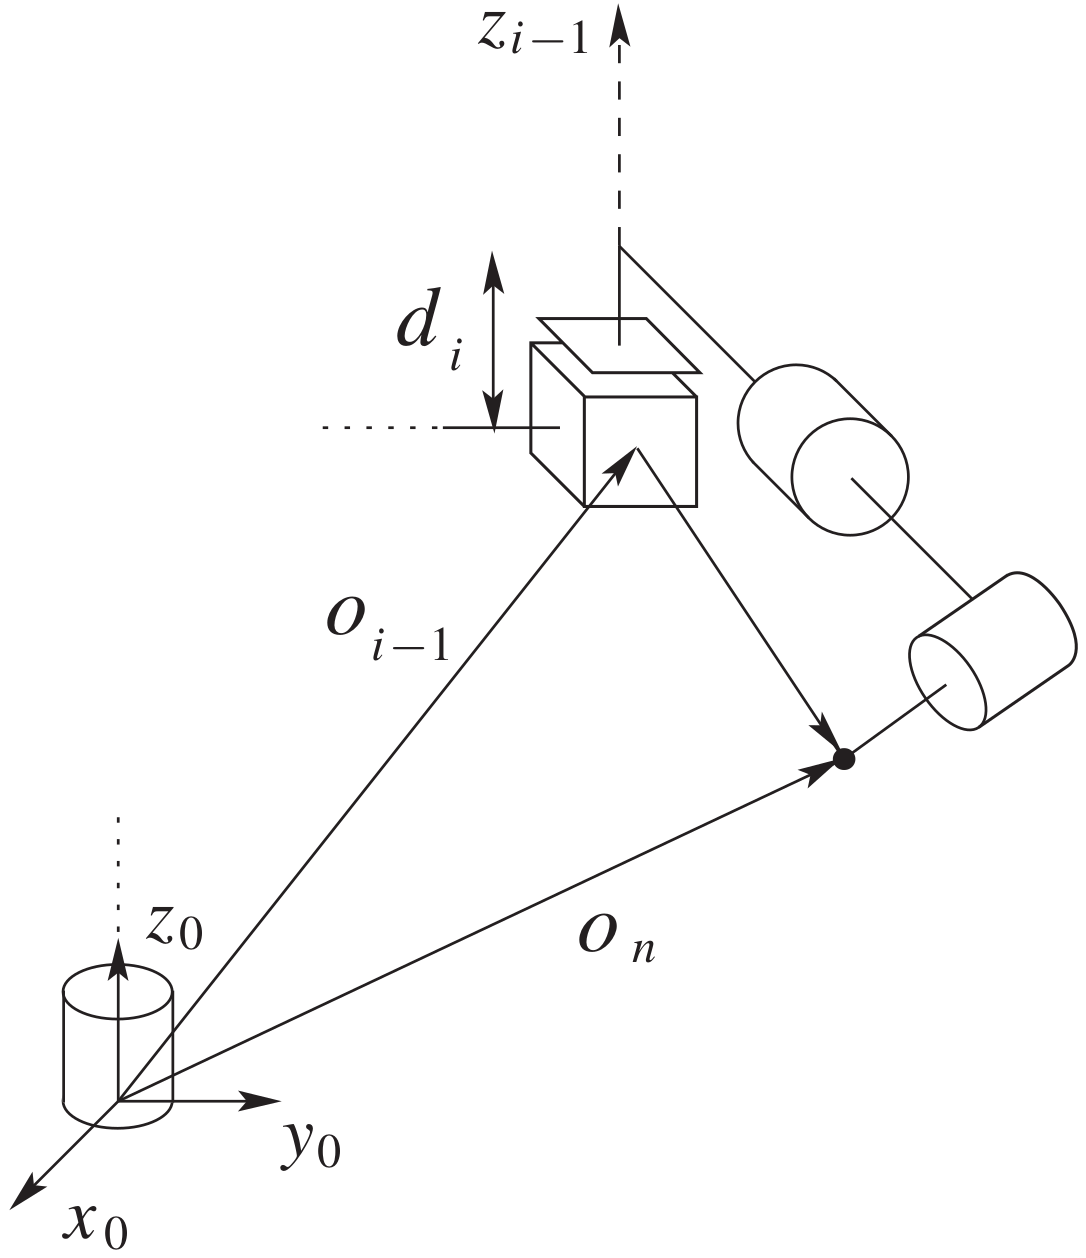
\includegraphics[width=0.95\textwidth]{figures/motion_due_to_prismatic.png} 
        %         % \caption{\footnotesize }
        %     \end{figure}
            % \vspace{-3mm}
        %     \centering
        %     \footnotesize{Motion of the end effector due to prismatic joint $i$.}
        % \end{column}
    % \end{columns}
\end{frame}


\begin{frame}
    \frametitle{Linear Velocity: Prismatic Joints}

    \begin{columns}
        \begin{column}{0.6\textwidth}
            \begin{itemize}
                \item Since joint $i$ is prismatic, it imparts a pure translation 
                to the end effector.
                \item The direction of this translation is $\parallel$ to
                $z_{i-1}$ and the magnitude is $\dot{d}_i$.
                \item Thus, expressed in $\Sigma_0$, we have
                \[ \dot{o}_n^0 = \dot{d}_iR_{i-1}^0\bmat{0 \\ 0 \\ 1} = \dot{d}_iz_{i-1}^0, \]
                in which $d_i$ is the joint variable for prismatic joint $i$.
                \item After dropping the superscripts, we have \[ J_{v_i} =
                z_{i-1}. \]
            \end{itemize}
        \end{column}
        \begin{column}{0.4\textwidth}
            \begin{figure}[bth]
                \centering
                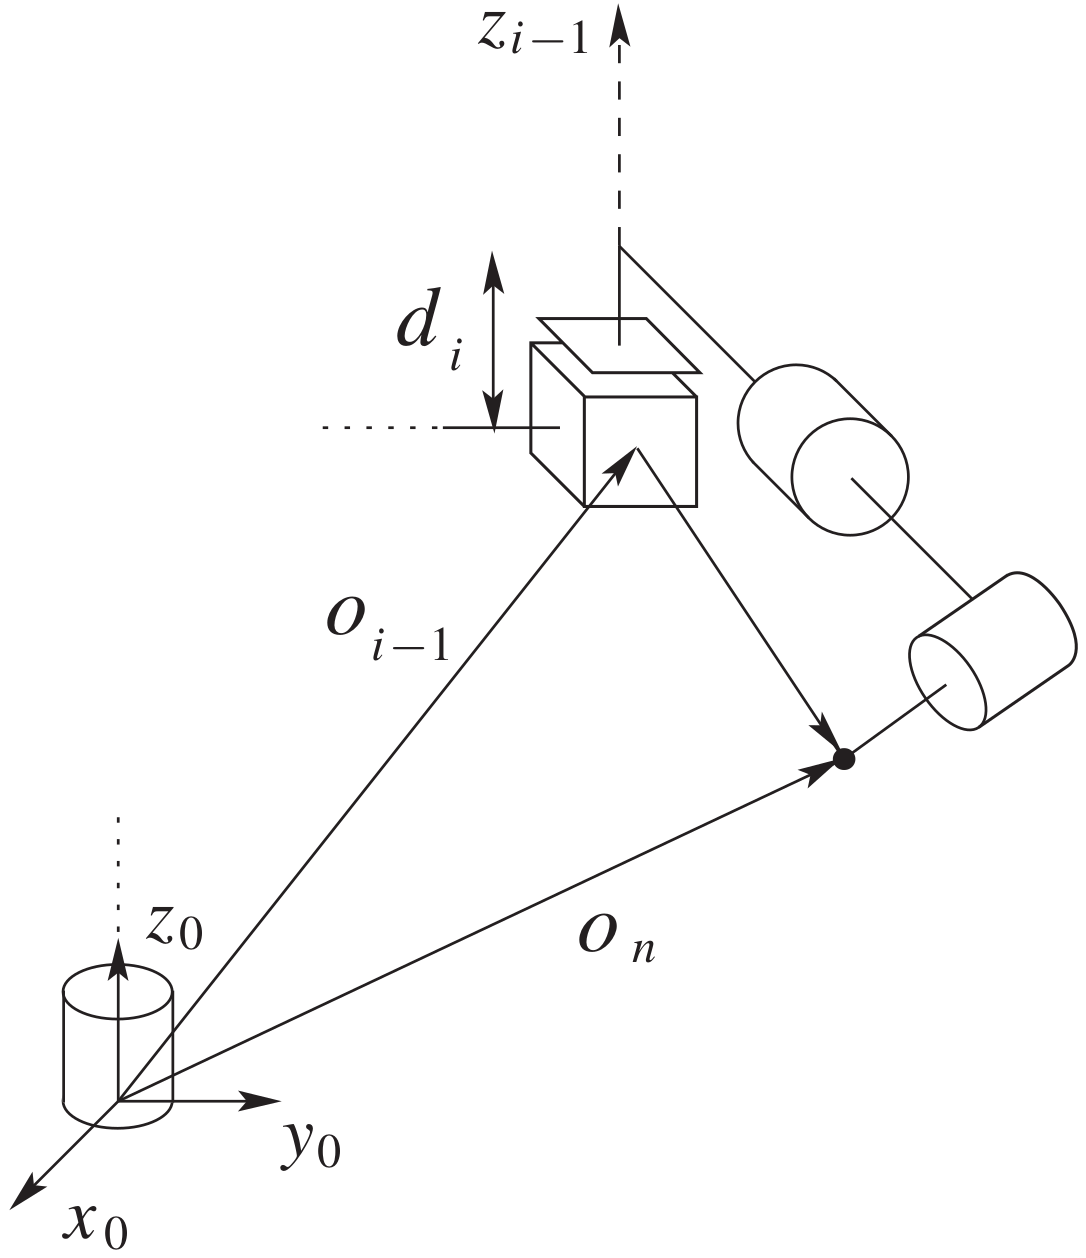
\includegraphics[width=0.95\textwidth]{figures/motion_due_to_prismatic.png} 
                % \caption{\footnotesize }
            \end{figure}
            \vspace{-3mm}
            \centering
            \footnotesize{Motion of the end effector due to prismatic joint $i$.}
        \end{column}
    \end{columns}
\end{frame}



\begin{frame}
    \frametitle{Linear Velocity: Revolute Joints}

    \begin{columns}
        \begin{column}{0.6\textwidth}
            \begin{itemize}
                \item Since joint $i$ is revolute, we have $q_i = \theta_i$.
                \item We see that the linear velocity of the end effector is
                simply of the form $\omega \times r$, where \[ \omega =
                \dot{\theta}_i z_{i-1}, \] and \[ r = o_n - o_{i-1}. \]
                \item Putting these together and expressing the coordinates
                relative to $\Sigma_0$, for a revolute joint we obtain
                \[ J_{v_i} = z_{i-1} \times (o_n - o_{i-1}). \]
            \end{itemize}
        \end{column}
        \begin{column}{0.4\textwidth}
            \begin{figure}[bth]
                \centering
                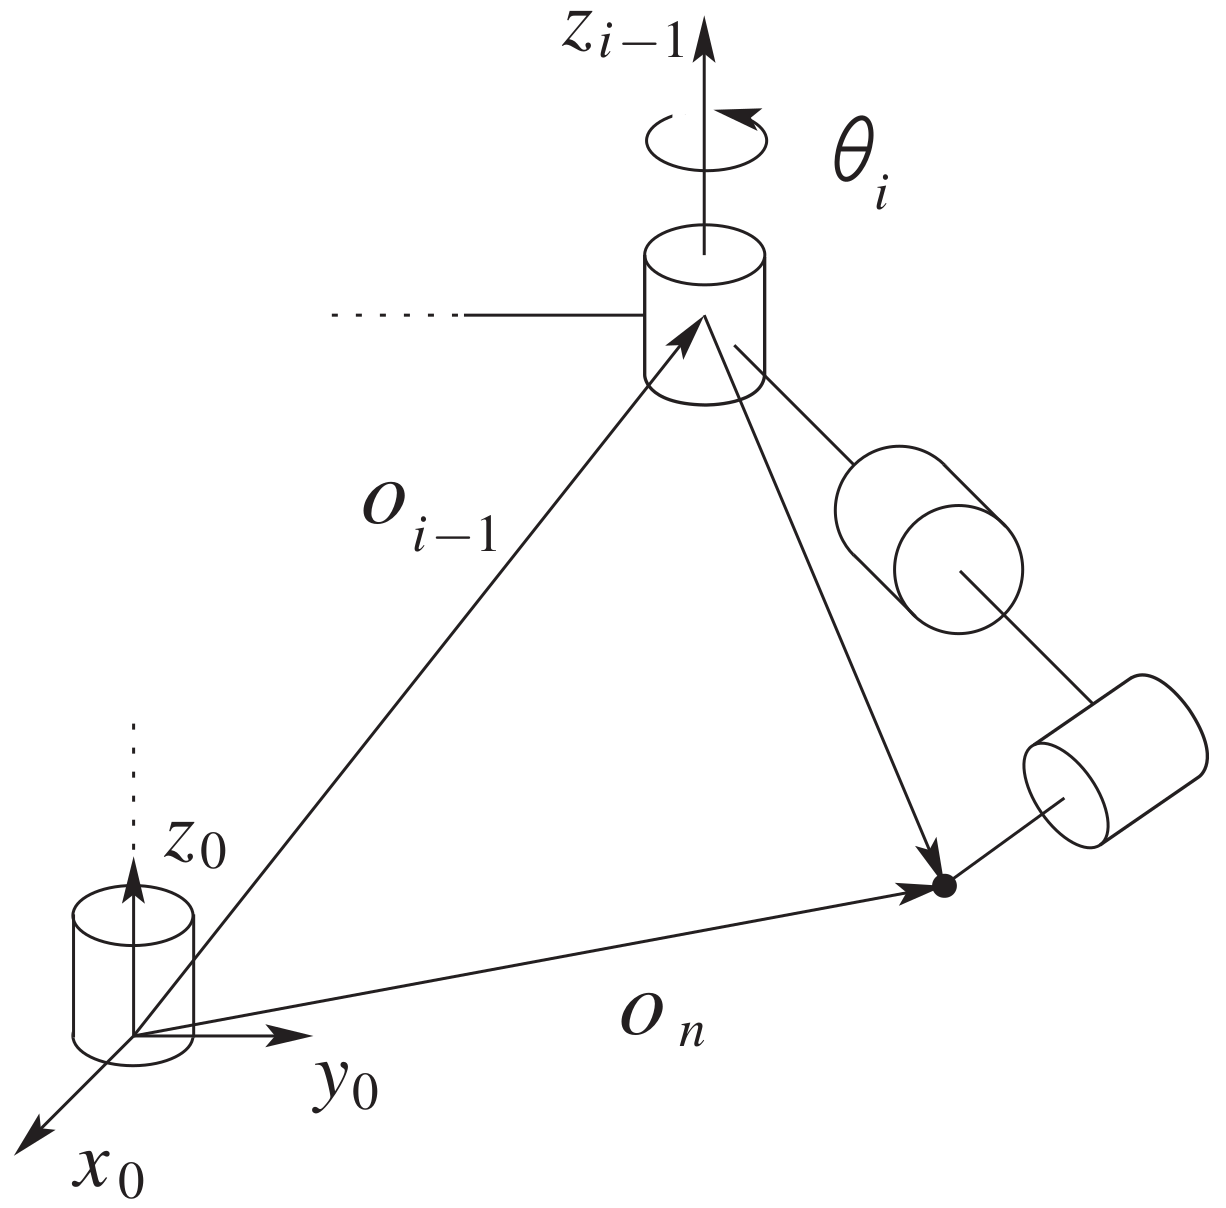
\includegraphics[width=0.95\textwidth]{figures/motion_due_to_revolute.png} 
                % \caption{\footnotesize }
            \end{figure}
            \vspace{-3mm}
            \centering
            \footnotesize{Motion of the end effector due to revolute joint $i$.}
        \end{column}
    \end{columns}
\end{frame}



\begin{frame}
    \frametitle{Combining Linear and Angular Velocity Jacobians}

    \begin{itemize}
        \item The upper half, $J_v$, of the Jacobian $J$ is given as \[ J_v =
        \bmat{J_{v_1} \cdots J_{v_n}}, \] in which the $i^{\textrm{th}}$ column
        $J_{v_i}$ is \[ J_{v_i} = 
        \begin{cases}
            z_{i-1} \times (o_n - o_{i-1}) & \mbox{for revolute joint $i$} \\
            z_{i-1} & \mbox{for prismatic joint $i$}
        \end{cases}    
        \]
        \item The lower half, $J_\omega$, of the Jacobian $J$ is given as
        \[J_\omega = \bmat{J_{\omega_1} \cdots J_{\omega_n}} \] in which the
        $i^{\textrm{th}}$ column $J_{\omega_i}$ is \[ J_{\omega_i} = 
        \begin{cases}
            z_{i-1} & \mbox{for revolute joint $i$} \\
            0 & \mbox{for prismatic joint $i$}
        \end{cases}
        \]
    \end{itemize}
\end{frame}


\begin{frame}
    \frametitle{Combining Linear and Angular Velocity Jacobians}

    \begin{itemize}
        \item The only quantities needed to compute the Jacobian are the unit 
        vectors $z_i$ and the coordinates of the origin $o_1, \ldots, o_n$.
        \item The coordinates for $z_i$ w.r.t. $\Sigma_0$ are given by the first 
        three elements in the third column of $T_i^0$.
        \item $o_i$ is given by the first three elements of the fourth column of 
        $T_i^0$.
        \item This procedure works not only for computing the velocity of the
        end effector but also for computing the velocity of any point on the
        manipulator.
    \end{itemize}
\end{frame}


\begin{frame}
    \frametitle{Example 4.5: Two-Link Planar Manipulator}
    \begin{columns}
        \begin{column}{0.6\textwidth}
            \only<1>{
            \begin{itemize}
                \item Since both joints are revolute, the Jacobian matrix is of the form
                \[
                J(q) = \bmat{
                    z_0 \times (o_2-o_0) & z_1 \times (o_2-o_1) \\ 
                    z_0 & z_1
                }    
                \]
                \item The various quantities are
                \[ z_0 = z_1 = \bmat{0 \\ 0 \\ 1}. \]
                \[
                o_0 = 0, \;\; o_1 = \bmat{a_1c_1 \\ a_1s_1 \\ 0}, \;\; o_2 = \bmat{
                    a_1c_1 + a_2c_{12} \\ a_1s_1 + a_2s_{12} \\ 0
                }
                \]
            \end{itemize}
            }
            \only<2>{
            \begin{itemize}
                \item The first two rows give the linear velocity of the origin 
                $o_2$ relative to the base.
                \item The third row is the linear velocity in the direction of
                $z_0$.
                \item The last three rows represent the angular velocity of the
                final frame, $\Sigma_2$, which is a basic rotation about the 
                vertical axis at the rate $\dot{\theta}_1 + \dot{\theta}_2$.
            \end{itemize}
            }
        \end{column}
        \begin{column}{0.4\textwidth}
            \begin{figure}[bth]
                \centering
                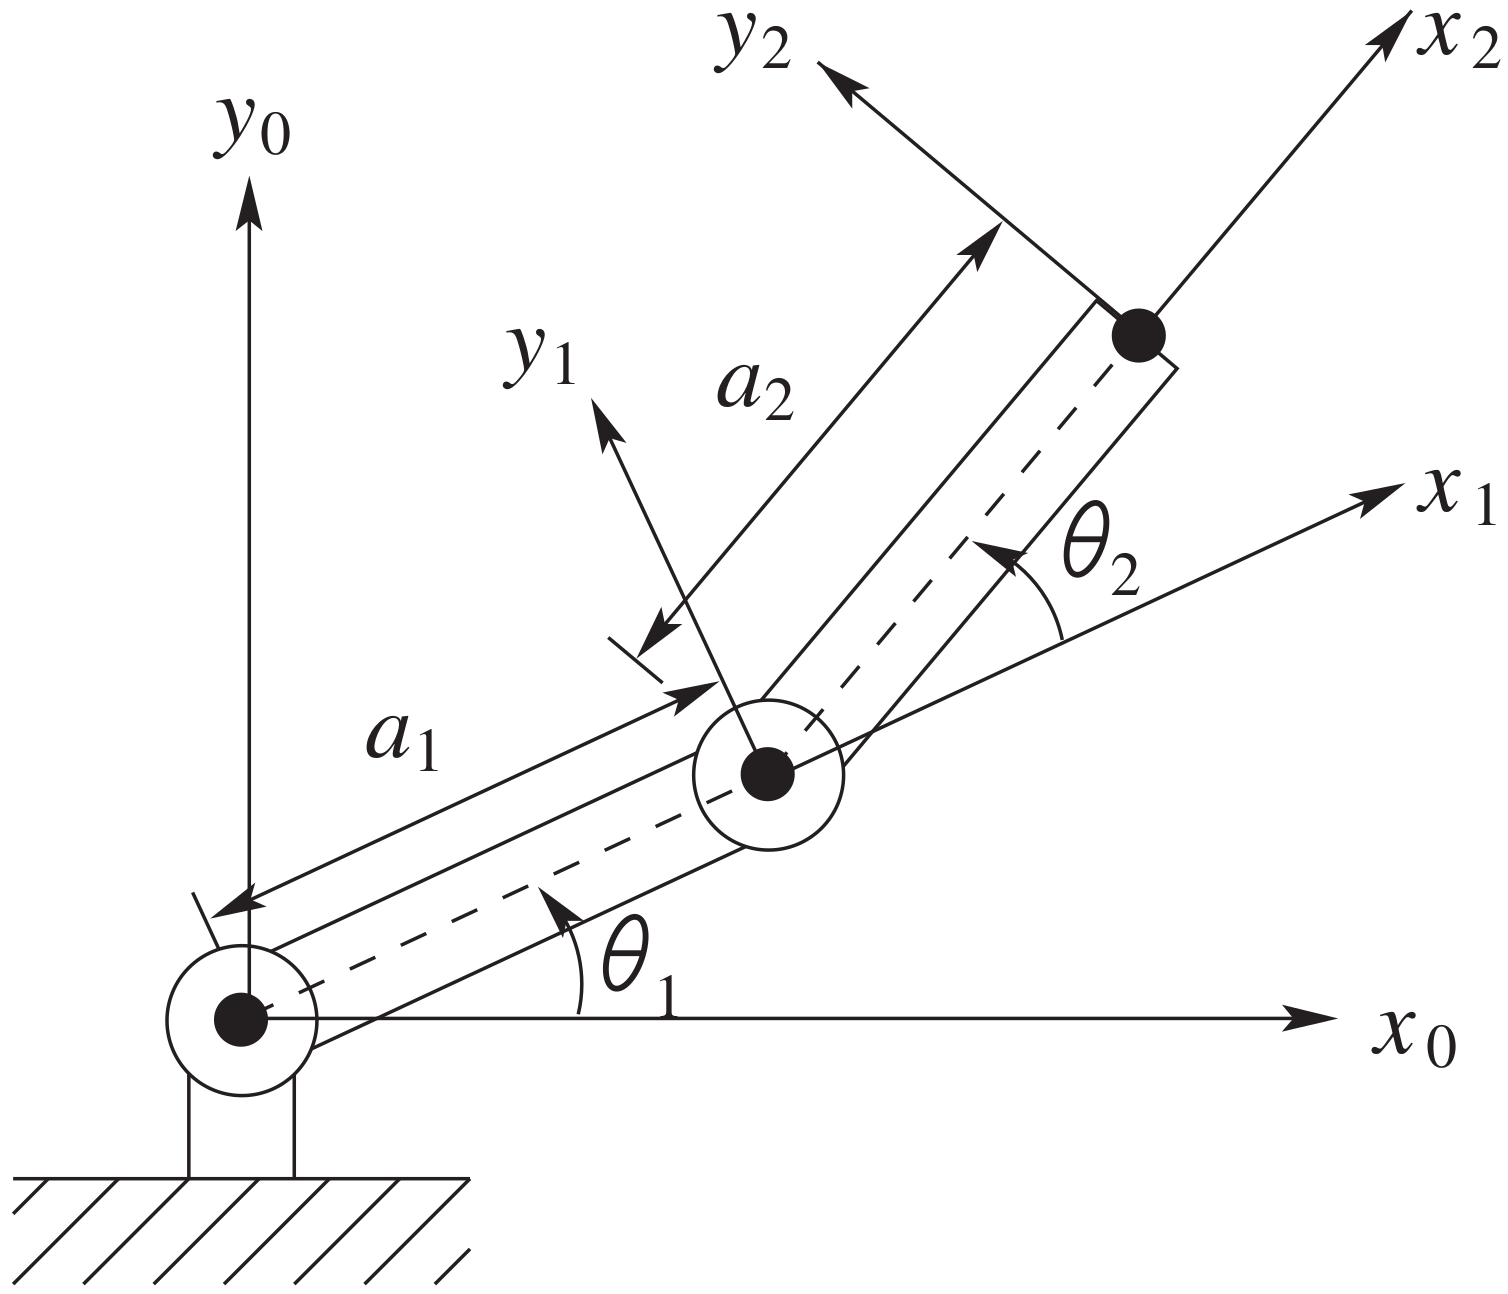
\includegraphics[width=0.85\textwidth]{figures/two_link_planar_manipulator.png} 
                % \caption{\footnotesize }
            \end{figure}
            \vspace{-2mm}
            \centering
            \footnotesize{Two-link planar manipulator.}
            \only<2>{
            \[
            J = \bmat{
                -a_1s_1 - a_2s_{12} & -a_2s_{12} \\
                a_1c_1 + a_2c_{12} & a_2c_{12} \\
                0 & 0 \\
                0 & 0 \\
                0 & 0 \\
                1 & 1
            }    
            \]
            }
        \end{column}
    \end{columns}
\end{frame}

\begin{frame}
    \frametitle{Example 4.6: Jacobian for an Arbitrary Point on a Link}
   
    \begin{columns}
        \begin{column}{0.6\textwidth}
            \only<1>{
            \begin{itemize}
                \item Suppose we wish to compute the linear velocity $v$ and the
                angular velocity $\omega$ of the center of link $2$ as shown.
                \[
                    \footnotesize{
                J(q) = \bmat{
                    z_0 \times (o_c-o_0) & z_1 \times (o_c-o_1) & 0 \\ 
                    z_0 & z_1 & 0
                }    
                    }
                \]
                which is merely the Jacobian with $o_c$ in place of $o_n$.
                \item The third column of the Jacobian is zero, since the
                velocity of the second link is unaffected by the motion of the 
                third link.
            \end{itemize}
            }
            % \only<2>{
            % \begin{itemize}
            %     \item The first two rows give the linear velocity of the origin 
            %     $o_2$ relative to the base.
            %     \item The third row is the linear velocity in the direction of
            %     $z_0$.
            %     \item The last three rows represent the angular velocity of the
            %     final frame, $\Sigma_2$, which is a basic rotation about the 
            %     vertical axis at the rate $\dot{\theta}_1 + \dot{\theta}_2$.
            % \end{itemize}
            % }
        \end{column}
        \begin{column}{0.4\textwidth}
            \begin{figure}[bth]
                \centering
                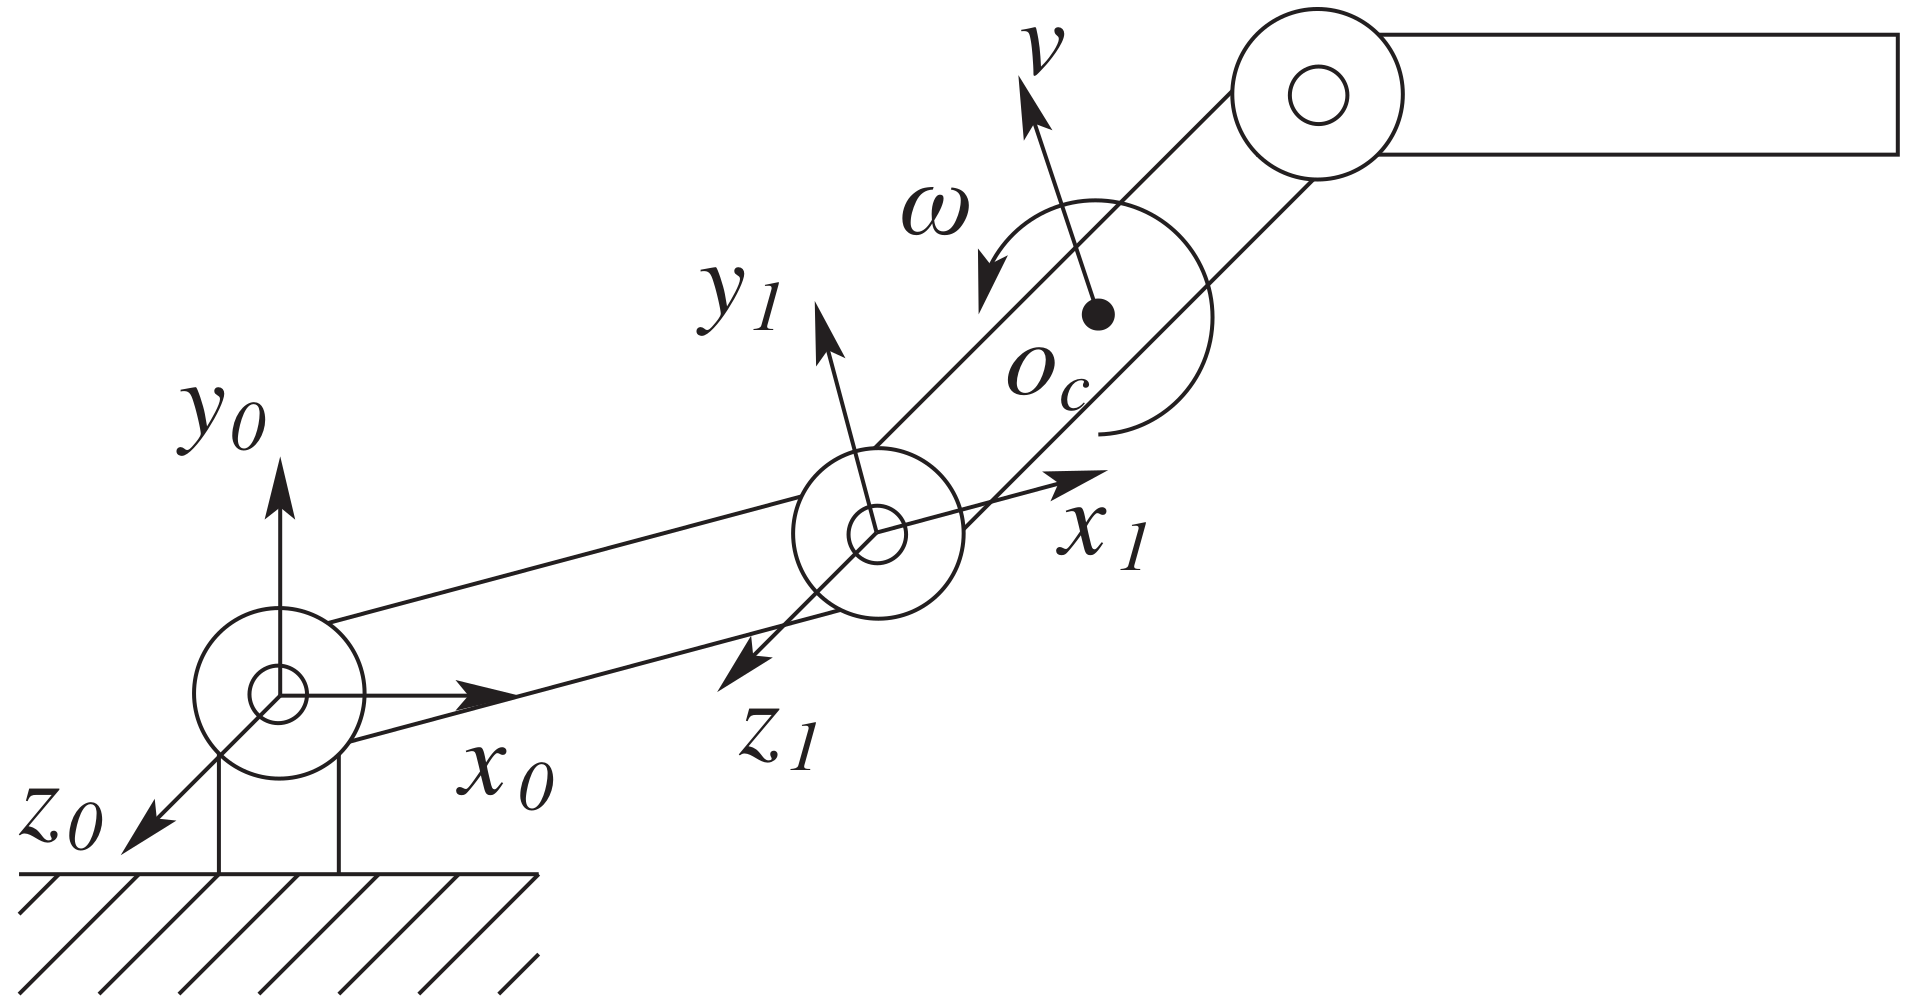
\includegraphics[width=0.85\textwidth]{figures/vel_of_planar_robot.png} 
                % \caption{\footnotesize }
            \end{figure}
            \vspace{-2mm}
            \centering
            \footnotesize{Finding the velocity of link $2$ of a $3$-link planar robot.}

            \begin{itemize}
                \item In this case the vector $o_c$ must be computed as it is 
                not given directy by the $T$ matrices.
            \end{itemize}
        \end{column}
    \end{columns}
\end{frame}

\begin{frame}
    \frametitle{Example 4.7: Stanford Manipulator}
   
    \begin{itemize}
        \item Joint $3$ is prismatic and $o_3 = o_4 = o_5$ as a consequence of 
        the spherical wrist and frame assignment.
        \item Denoting this common origin by $o$, we see that the columns of the 
        Jacobian have the form

        \begin{align*}
            J_i &= \bmat{z_{i-1} \times (o_6 - o_{i-1}) \\ z_{i-1}}, \; \; i = 1,2, \\
            J_3 &= \bmat{z_2 \\ 0} \\
            J_i &= \bmat{z_{i-1} \times (o_6 - o) \\ z_{i-1}}, \; \; i = 4,5,6.
        \end{align*}
    \end{itemize}
\end{frame}

\begin{frame}
    \frametitle{Example 4.8: SCARA Manipulator}
   
    \begin{itemize}
        \item This Jacobian is a $6 \times 4$ matrix since SCARA has only four 
        degrees of freedom.
        \item We need only compute the matrices $T_j^0 = A_1 \cdots A_j$.
        \item Since joints $1$, $2$, and $4$ are revolute and joint $3$ is
        prismatic, and since $o_4 - o_3 \parallel z_3$ (and thus $z_3 \times
        (o_4 - o_3) = 0$), the Jacobian is of the form
        \begin{align*}
        J &= \bmat{
            z_0 \times (o_4 - o_0) & z_1 \times (o_4 - o_1) & z_2 & 0 \\ 
            z_0 & z_1 & 0 & z_3
        } \\
        &= \bmat{
            -a_1s_1 - a_2s_{12} & -a_2s_{12} & 0 & 0 \\
            a_1c_1 + a_2c_{12} & a_2c_{12} & 0 & 0 \\
            0 & 0 & -1 & 0 \\
            0 & 0 & 0 & 0 \\
            0 & 0 & 0 & 0 \\
            1 & 1 & 0 & -1
        }.
        \end{align*}
    \end{itemize}

\end{frame}

\endgroup
% \section{The Tool Velocity}

\begin{frame}[standout, plain, noframenumbering]
    The Tool Velocity

    % \medskip

    % \footnotesize
    % Sam Greydanus \quad Misko Dzamba \quad Jason Yosinski
\end{frame}

\begingroup
\small

\begin{frame}
    \frametitle{The Tool Velocity}

    \begin{itemize}
        \item Many tasks require that a tool be attached to the end effector.
        \item It is necessary to relate the velocity of the tool frame to the 
        velocity of the end-effector frame.
        \item The fixed spatial relationship between the end effector and the 
        tool frame is given by the constant homogeneous transformation matrix 
        \[
        T_{\textrm{tool}}^n = \bmat{R & d \\ 0 & 1}.
        \]
        \item We assume that the end effector velocity is given and expressed in
        the end effector frame $\Sigma_n$, i.e., we are given $\xi_n^n$.
        \item We will derive the velocity of the tool expressed in coordinates
        relative to the tool frame, that is, we will derive
        $\xi_{\textrm{tool}}^{\textrm{tool}}$.
    \end{itemize}
\end{frame}



\begin{frame}
    \frametitle{The Tool Velocity}

    \begin{itemize}
        \item Since the two frames are rigidly attached, the angular velocity of
        the tool frame is the same as the angular velocity of the end-effector
        frame. Indeed, we have $R_{\textrm{tool}}^0 = R_n^0R$, with $R$ constant
        \[
            \dot{R}_{\textrm{tool}}^0 = \dot{R}_n^0R \Longrightarrow 
            S\left( \omega_{\textrm{tool}}^0 \right)R_{\textrm{tool}}^0 = S\left( \omega_n^0 \right)R_n^0R
            \Longrightarrow \omega_{\textrm{tool}} = \omega_n.
        \]
        \item To obtain the tool angular velocity relative to the tool frame, we
        apply a rotational transformation \[
        \omega_{\textrm{tool}}^{\textrm{tool}} = \omega_n^{\textrm{tool}} =
        R^\top \omega_n^n. \]
        \item If the end-effector frame is moving with body velocity $\xi =
        (v_n, \omega_n)$, then the linear velocity of the origin of the tool
        frame, which is rigidly attached to the end-effector frame, is given by
        \[ v_{\textrm{tool}} = v_n + \omega_n \times r, \] where $r$ is the
        vector from the origin of $\Sigma_n$ to the origin of
        $\Sigma_{\textrm{tool}}$.
    \end{itemize}
\end{frame}


\begin{frame}
    \frametitle{The Tool Velocity}

    \begin{itemize}
        \item We can express $r$ in coordinates relative to
        $\Sigma_{\textrm{tool}}$ as $r^{\textrm{tool}} = R^\top d$.
        \item Thus, we can write 
        \begin{align*}
            \omega_n^{\textrm{tool}} \times r^{\textrm{tool}} &= 
            R^\top \omega_n^n \times \left( R^\top d \right) = -R^\top d \times 
            R^\top \omega_n^n = -S\left( R^\top d \right)R^\top \omega_n^n \\
            &= R^\top S(d) RR^\top \omega_n^n = -R^\top S(d) \omega_n^n.
        \end{align*}
        \item We express the free vector $v_n^n$ in coordinates relative to
        $\Sigma_{\textrm{tool}}$ \[v_n^{\textrm{tool}} = R^\top v_n^n. \]
        \item Combining, we obtain
        \begin{align*}
            v_{\textrm{tool}}^{\textrm{tool}} &= R^\top v_n^n - R^\top S(d) \omega_n^n, \\
            \omega_{\textrm{tool}}^{\textrm{tool}} &= R^\top \omega_n^n.
        \end{align*}
        which can be expressed as the matrix equation
        \[
        \xi_{\textrm{tool}}^{\textrm{tool}} = \bmat{R^\top & -R^\top S(d) \\ 0_{3 \times 3} & R^\top}\xi_n^n.
        \]
    \end{itemize}
\end{frame}


\begin{frame}
    \frametitle{The Tool Velocity}

    \begin{itemize}
        \item In many cases, it is useful to solve the inverse problem: compute
        the required end effector velocity to produce a desired tool velocity.
        Since 
        \[
        \bmat{R & S(d)R \\ 0 & R} = \bmat{R^\top & -R^\top S(d) \\ 0 & R^\top}^{-1}
        \]
        we can solve the equation above for $\xi_n^n$, obtaining
        \[ \omega_n^n = \bmat{R & S(d)R \\ 0 & R}\xi_{\textrm{tool}}^{\textrm{tool}}. \]
        \item This gives the general expression for transforming velocities
        between two rigidly attached moving frames
        \[
        \xi_A^A = \bmat{R_B^A & S\left( d_B^A \right)R_B^A \\ 0 & R_B^A}\xi_B^B.
        \]
    \end{itemize}
\end{frame}


\endgroup
% \section{The Analytical Jacobian}

\begin{frame}[standout, plain, noframenumbering]
    The Analytical Jacobian

    % \medskip

    % \footnotesize
    % Sam Greydanus \quad Misko Dzamba \quad Jason Yosinski
\end{frame}

\begingroup
\small



\begin{frame}
    \frametitle{The Analytical Jacobian}

    \begin{itemize}
        \item The Jacobian matrix derived above is sometimes called the
        \textbf{geometric Jacobian} to distinguish from the \textbf{analytical
        Jacobian}, denoted $J_a(q)$. Let \[ X = \bmat{d(q) \\ \alpha(q)} \]
        denote the end effector pose
        \begin{itemize}
            \footnotesize{
            \item $d(q)$ is the usual vector from the origin of the base frame to the origin of the end-effector frame,
            \item $\alpha(q)$ denotes a minimal representation for the orientation of the end effector frame relative to the base frame.
            }
        \end{itemize} 
        \item Let $\alpha = (\phi, \theta, \psi)$ be a vector of Euler angles.
        Then, we seek an expression of the form \[ \dot{X} = \bmat{\dot{d} \\
        \dot{\alpha}} = J_a(q)\dot{q} \] to define the analytical Jacobian.
    \end{itemize}
\end{frame}


\begin{frame}
    \frametitle{The Analytical Jacobian}

    \begin{itemize}
        \item It can be shown that, if $R = R_{z,\phi}R_{y,\theta}R_{z,\psi}$ is 
        the Euler angle transformation, then \[ \dot{R} = S(\omega)R \] in which 
        $\omega$ defining the angular velocity is given by
        \[
        \omega = \bmat{c_\psi s_\theta \dot{\phi} - s_\psi \dot{\theta} \\ 
                    s_\psi s_\theta \dot{\phi} + c_\psi \dot{\theta} \\ 
                    \dot{\psi} + c_\theta \dot{\phi}} = 
        \bmat{
            c_\psi s_\theta & -s_\psi & 0 \\ s_\psi s_\theta & c_\psi & 0 \\ 
            c_\theta & 0 & 1
        }\bmat{\dot{\phi} \\ \dot{\theta} \\ \dot{\psi}} = B(\alpha)\dot{\alpha}.
        \]
        \item The components of $\omega$ are called \textbf{nutation},
        \textbf{spin}, and \textbf{precession}.
        \item Combining the above relationships with the previous definition
        yields
        \[
        J(q)\dot{q} = \bmat{v \\ \omega} = \bmat{\dot{d} \\ B(\alpha)\dot{\alpha}}
        = \bmat{I & 0 \\ 0 & B(\alpha)}\bmat{\dot{d} \\ \dot{\alpha}} = \bmat{I & 0 \\ 0 & B(\alpha)}J_a(q)\dot{q}.
        \]
    \end{itemize}
\end{frame}


\begin{frame}
    \frametitle{The Analytical Jacobian}

    \begin{itemize}
        \item Thus, the analytical Jacobian, $J_a(q)$, may be computed from the 
        geometric Jacobian as
        \[ J_a(q) = \bmat{I & 0 \\ 0 & B^{-1}(\alpha)}J(q), \]
        provided that $\det B(\alpha) \neq 0$.
        \item In the next section, we discuss the notion of Jacobian
        singularities, which are configurations where the Jacobian loses rank.
        \item Singularities of the matrix $B(\alpha)$ are called
        \textbf{representation singularities}.
        \item It can be easily shown that $B(\alpha)$ is invertible provided
        that $s_\theta \neq 0$.
        \item The singularities of the analytical Jacobian include the
        singularities of the geometric Jacobian, $J$, together with the 
        representational singularities.
    \end{itemize}
\end{frame}


\endgroup
% \section{Singularities}

\begin{frame}[standout, plain, noframenumbering]
    Singularities

    % \medskip

    % \footnotesize
    % Sam Greydanus \quad Misko Dzamba \quad Jason Yosinski
\end{frame}

\begingroup
\small


\begin{frame}
    \frametitle{Singularities}

    \begin{itemize}
        \item The $6 \times n$ Jacobian $J(q)$ defines a mapping \[ \xi =
        J(q)\dot{q} \] between the vector $\dot{q}$ of joint velocities and the
        vector $\xi = (v, \omega)$ of end effector velocities. In other words,
        \[ \xi = J_1 \dot{q}_1 + J_2 \dot{q}_2 + \cdots + J_n \dot{q}_n. \]
        \item Since $\xi \in \mathbb{R}^6$, it is necessary that $J$ have six 
        linearly independent columns for the end effector to be able to achieve 
        any arbitrary velocity.
        \item Thus, when $\rank J = 6$, the end effector can execute any
        arbitrary velocity. Notice that for a matrix $J \in \mathbb{R}^{6 \times
        n}$, it is always the case that $\rank J \leq \min{(6, n)}$.
    \end{itemize}
\end{frame}


\begin{frame}
    \frametitle{Singularities}

    \begin{itemize}
        \item The rank of the manipulator Jacobian will depend on the
        configuration $q$.
        \item Configurations for which $\rank J(q)$ is less than its maximum
        value are called \textbf{singularities} or \textbf{singular
        configurations}.
        \item Identifying manipulator singularities is important because \ldots
        \begin{itemize}
            \footnotesize{
            \item Singularities represent configurations from which certain
            directions of motion may be unattainable.
            \item At singularities, bounded end effector velocities may
            correspond to unbounded joint velocities.
            \item At singularities, bounded joint torques may correspond to
            unbounded end effector forces and torques.
            \item Singularities often correspond to poitns on the boundary of
            the manipulator workspace, that is, to points of maximum reach of
            the manipulator.
            \item Singularities correspond to points in the manipulator
            workspace that may be unreachable under small perturbations of the
            link parameters, such as length, offset, etc.
            }
        \end{itemize}
    \end{itemize}
\end{frame}


\begin{frame}
    \frametitle{Decoupling of Singularities}

    \begin{itemize}
        \item For manipulators with spherical wrists, determination of singular
        configurations may be decoupled into two simpler problems.
        \item The first problem is to determine so-called \textbf{arm
        singularities}, that is, singularities resulting from the motion of the
        arm, which consists of the first three or more links.
        \item The second problem is to determine the \textbf{wrist
        singularities} resulting from motion of the spherical wrist.
    \end{itemize}
\end{frame}


\begin{frame}
    \frametitle{Decoupling of Singularities}

    \begin{itemize}
        \item Consider the case that $n=6$, that is, the manipulator consists of 
        a $3$-DOF arm with a $3$-DOF spherical wrist.
        \item The Jacobian is a $6 \times 6$ matrix and a configuration $q$ is
        singular iff $\det J(q) = 0$.
        \item If we partition the Jacobian into $3 \times 3$ blocks as 
        \[ J = \begin{bNiceArray}{c|c}
            J_P & J_O
        \end{bNiceArray} = 
        \begin{bNiceArray}{c|c}[margin]
            J_{11} & J_{12} \\ \hline
            J_{21} & J_{22}
        \end{bNiceArray} 
        \]
        then, since the final three joints are always revolute
        \[
        J_O = \bmat{
            z_3 \times (o_6 - o_3) & z_4 \times (o_6 - o_4) & z_5 \times (o_6 - o_5) \\
            z_3 & z_4 & z_5
        }    
        \]
    \end{itemize}
\end{frame}

\begin{frame}
    \frametitle{Decoupling of Singularities}

    \begin{itemize}
        \item Since the wrist axes intersect at a common point $o$, if we choose
        the coordinate frames so that $o_3 = o_4 = o_5 = o_6 = o$, then $J_O$
        becomes
        \[
        J_O = \bmat{0 & 0 & 0 \\ z_3 & z_4 & z_5}    
        \]
        \item In this case, the Jacobian matrix has the block triangular form 
        \[ J = \begin{bNiceArray}{c|c}[margin]
            J_{11} & 0 \\ \hline
            J_{21} & J_{22}
        \end{bNiceArray}  \]
        with determinant \[ \det J = \det J_{11} \det J_{22}. \]
        \item $J_{11}$ has $i^{\textrm{th}}$ column $z_{i-1} \times (o -
        o_{i-1})$ if joint $i$ is revolute, and $z_{i-1}$if joint $i$ is
        prismatic, while \[ J_{22} = \bmat{z_3 & z_4 & z_5}. \]
    \end{itemize}
\end{frame}


\begin{frame}
    \frametitle{Decoupling of Singularities}

    \begin{itemize}
        \item Therefore, the set of singular configurations of the manipulator is 
        the set of arm configurations satisfying $\det J_{11} = 0$
        \item and the set of wrist configurations satisfying $\det J_{22} = 0$.
        \item This form of the Jacobian does not necessarily give the correct
        relation between the velocity of the end effector and the joint
        velocities.
        \item It is intended only to simplify the determination of
        singularities.
    \end{itemize}
\end{frame}



\begin{frame}
    \frametitle{Wrist Singularities}

    \begin{columns}
        \begin{column}{0.6\textwidth}
            \begin{itemize}
                \item A spherical wrist is in a singular configuration whenever the
                vectors $z_3$, $z_4$, and $z_5$ that make up $J_{22} = \bmat{z_3 & z_4 &
                z_5}$ are linearly dependent.
                \item Referring to the figure, we see that this happens when the 
                joint axes $z_3 \parallel z_5$, that is, when $\theta_5 = 0$ or $\pi$.
                \item These are the only singularities of the spherical wrist, and 
                they are unavoidable w/o imposing mechanical limits.
            \end{itemize}
        \end{column}
        \begin{column}{0.4\textwidth}
            \begin{figure}[bth]
                \centering
                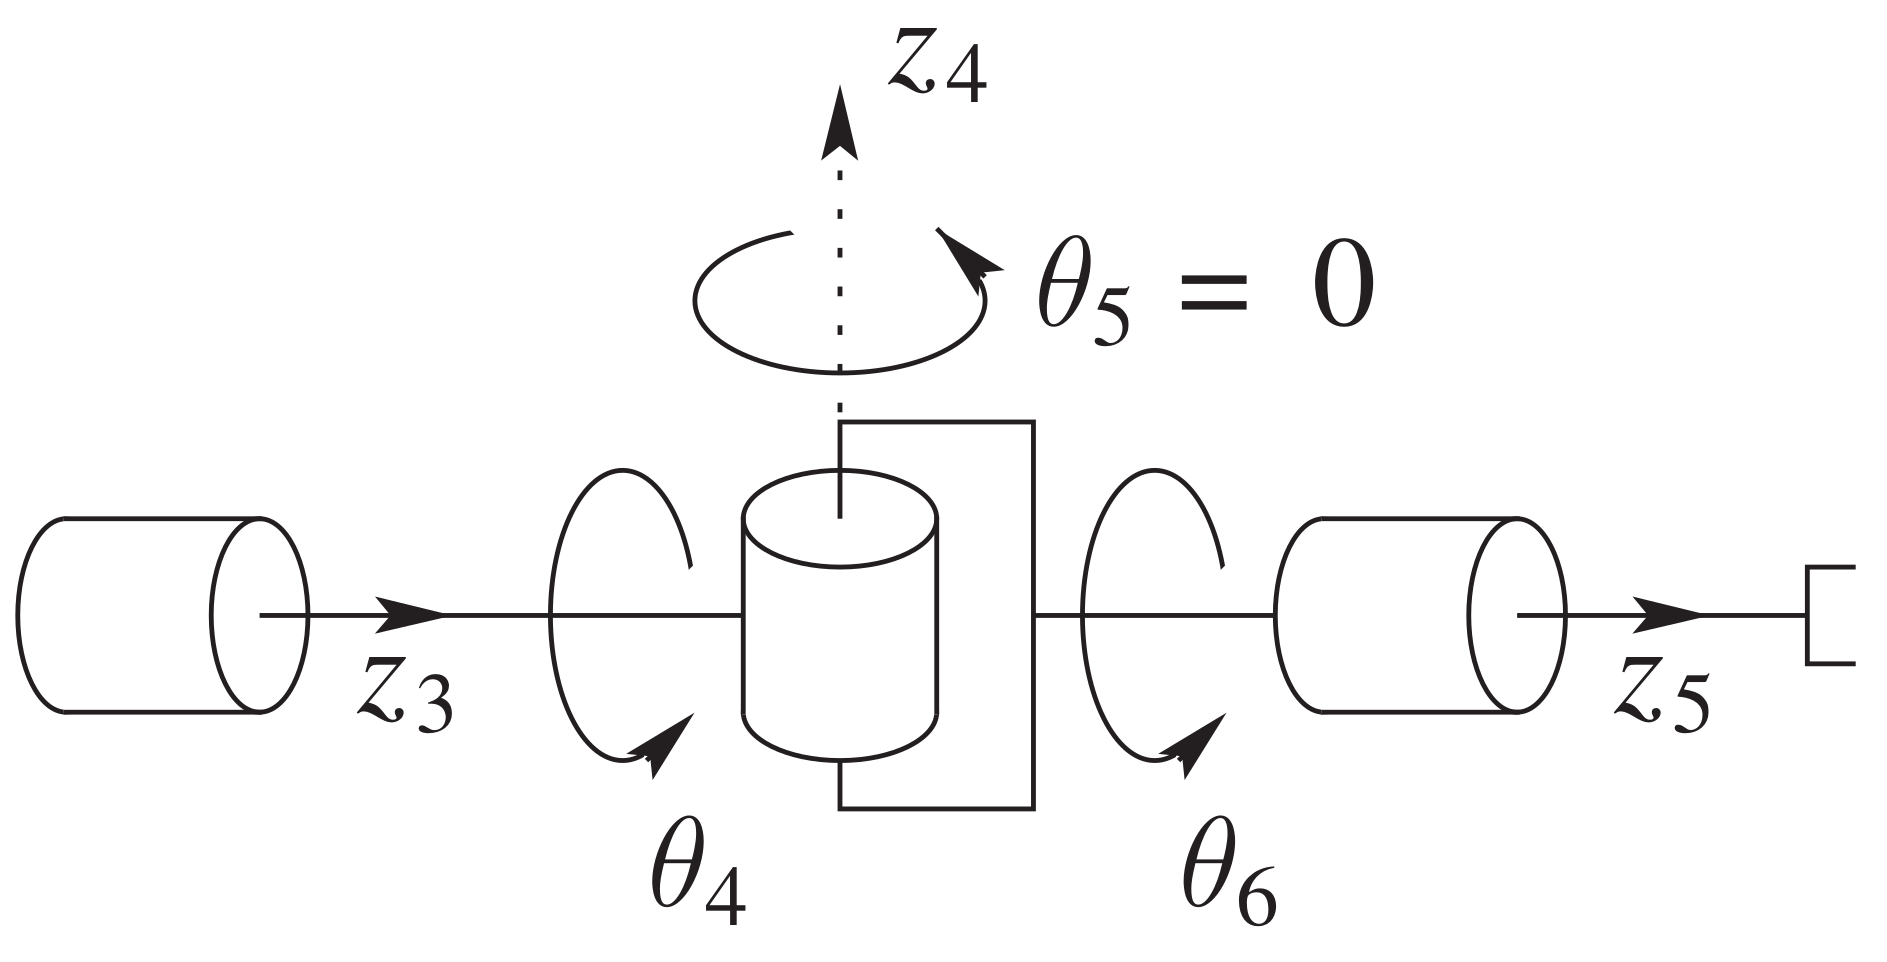
\includegraphics[width=0.85\textwidth]{figures/spherical_wrist_singularity.png} 
                % \caption{\footnotesize }
            \end{figure}
            \vspace{-2mm}
            \centering
            \footnotesize{Spherical wrist singularity}
        \end{column}
    \end{columns}
\end{frame}



\begin{frame}
    \frametitle{Arm Singularities}

    \begin{itemize}
        \item To investigate arm singularities we need only to compute $\det
        J_{11}$, which is done using the equation
        \[ J_{v_i} = 
        \begin{cases}
            z_{i-1} \times (o - o_{i-1}) & \mbox{for revolute joint $i$} \\
            z_{i-1} & \mbox{for prismatic joint $i$}
        \end{cases}    
        \]
        where $o$ is the wrist center.
    \end{itemize}
\end{frame}


\begin{frame}
    \frametitle{Arm Singularities of Elbow Manipulator}

    \begin{itemize}
        \item The three-link articulated manipulator has the determinant $J_{11}$
        \[
            J_{11} = \bmat{
                -a_2s_1c_2 - a_3s_1c_{23} & -a_2s_2c_1 - a_3s_{23}c_1 & -a_3c_1s_{23} \\ 
                a_2c_1c_2 + a_3c_1c_{23} & -a_2s_1s_2 - a_3s_1s_{23} & -a_3s_1s_{23} \\ 
                0 & a_2c_2 + a_3c_{23} & a_3c_{23}
            }
        \]
    \end{itemize}
    \begin{columns}
        \begin{column}{0.6\textwidth}
            \begin{itemize}
                \item The determinant of $J_{11}$ is 
                \[ \det J_{11} = -a_2a_3s_3(a_2c_2 + a_3c_{23}). \]
            \end{itemize}
        \end{column}
        \begin{column}{0.4\textwidth}
            \begin{figure}[bth]
                \centering
                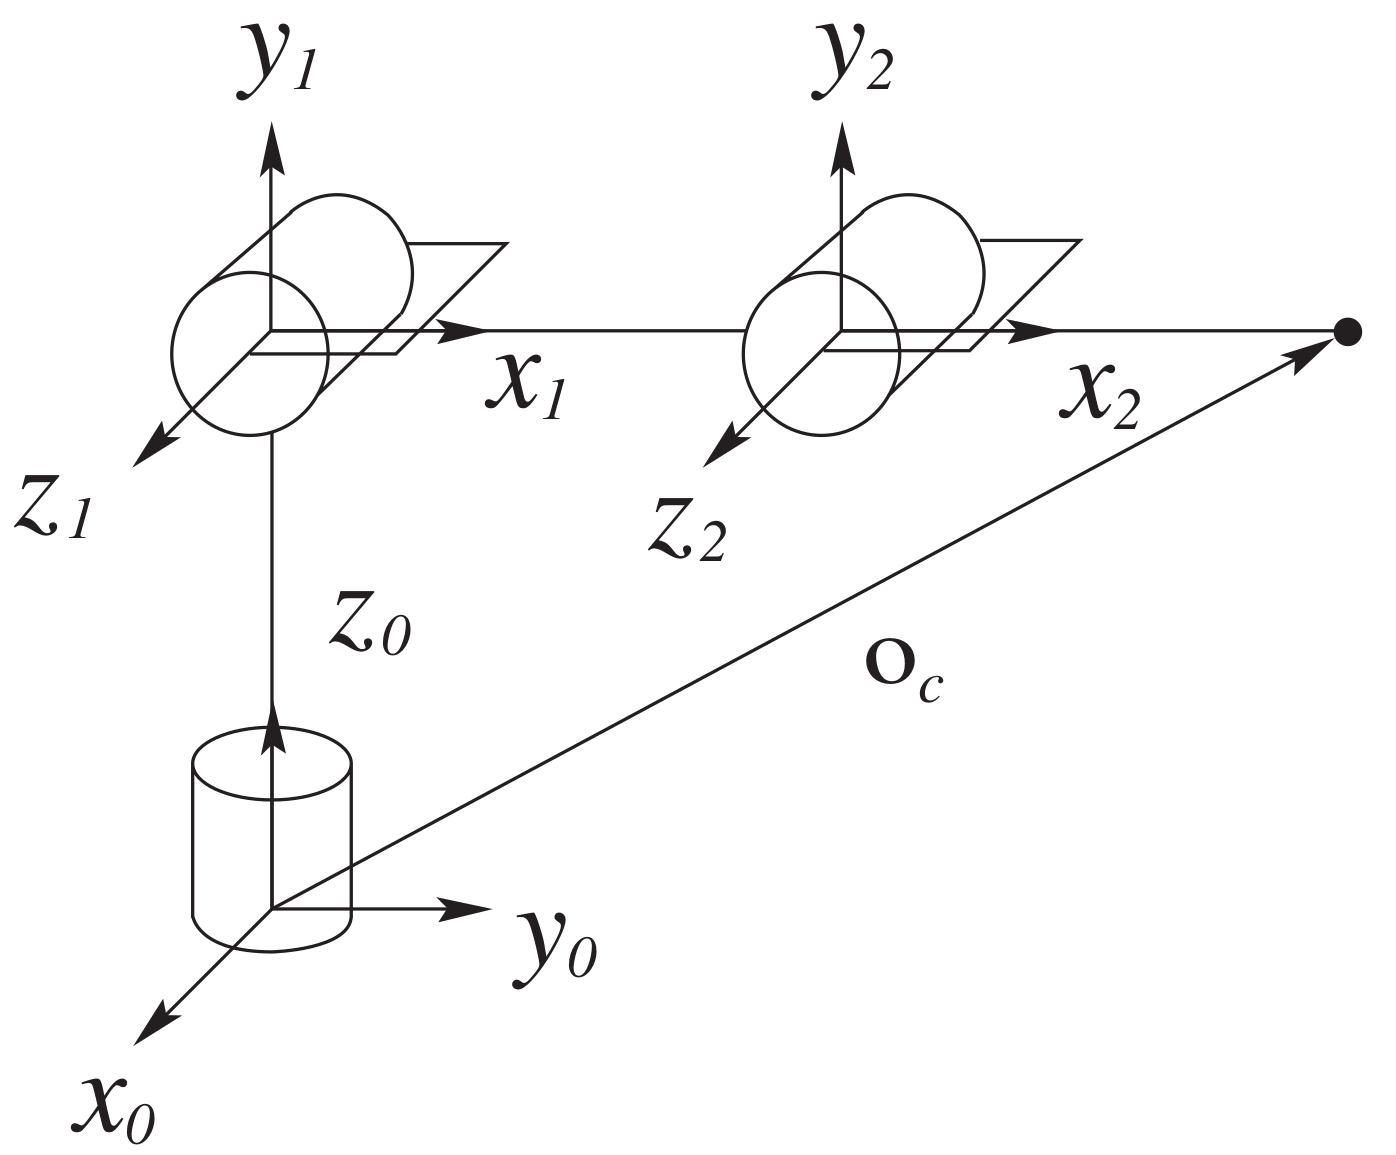
\includegraphics[width=0.85\textwidth]{figures/elbow_manipulator_sing.png} 
                % \caption{\footnotesize }
            \end{figure}
            \vspace{-2mm}
            \centering
            \footnotesize{Elbow manipulator}
        \end{column}
    \end{columns}
\end{frame}


\begin{frame}
    \frametitle{Arm Singularities of Elbow Manipulator}

    \begin{columns}
        \begin{column}{0.6\textwidth}
            \begin{itemize}
                \item We see that the elbow manipulator is
                in a singular configuration when
                \[ s_3 = 0 \Longrightarrow \theta_3 = 0, \pi. \]
                and whenever
                \[ a_2c_2 + a_3c_{23} = 0. \]
                \item The situation of $\theta_3 = 0, \pi$ arises when the elbow
                is fully extended or retracted as shown on the bottom right
                figure.
            \end{itemize}
        \end{column}
        \begin{column}{0.4\textwidth}
            \begin{figure}[bth]
                \centering
                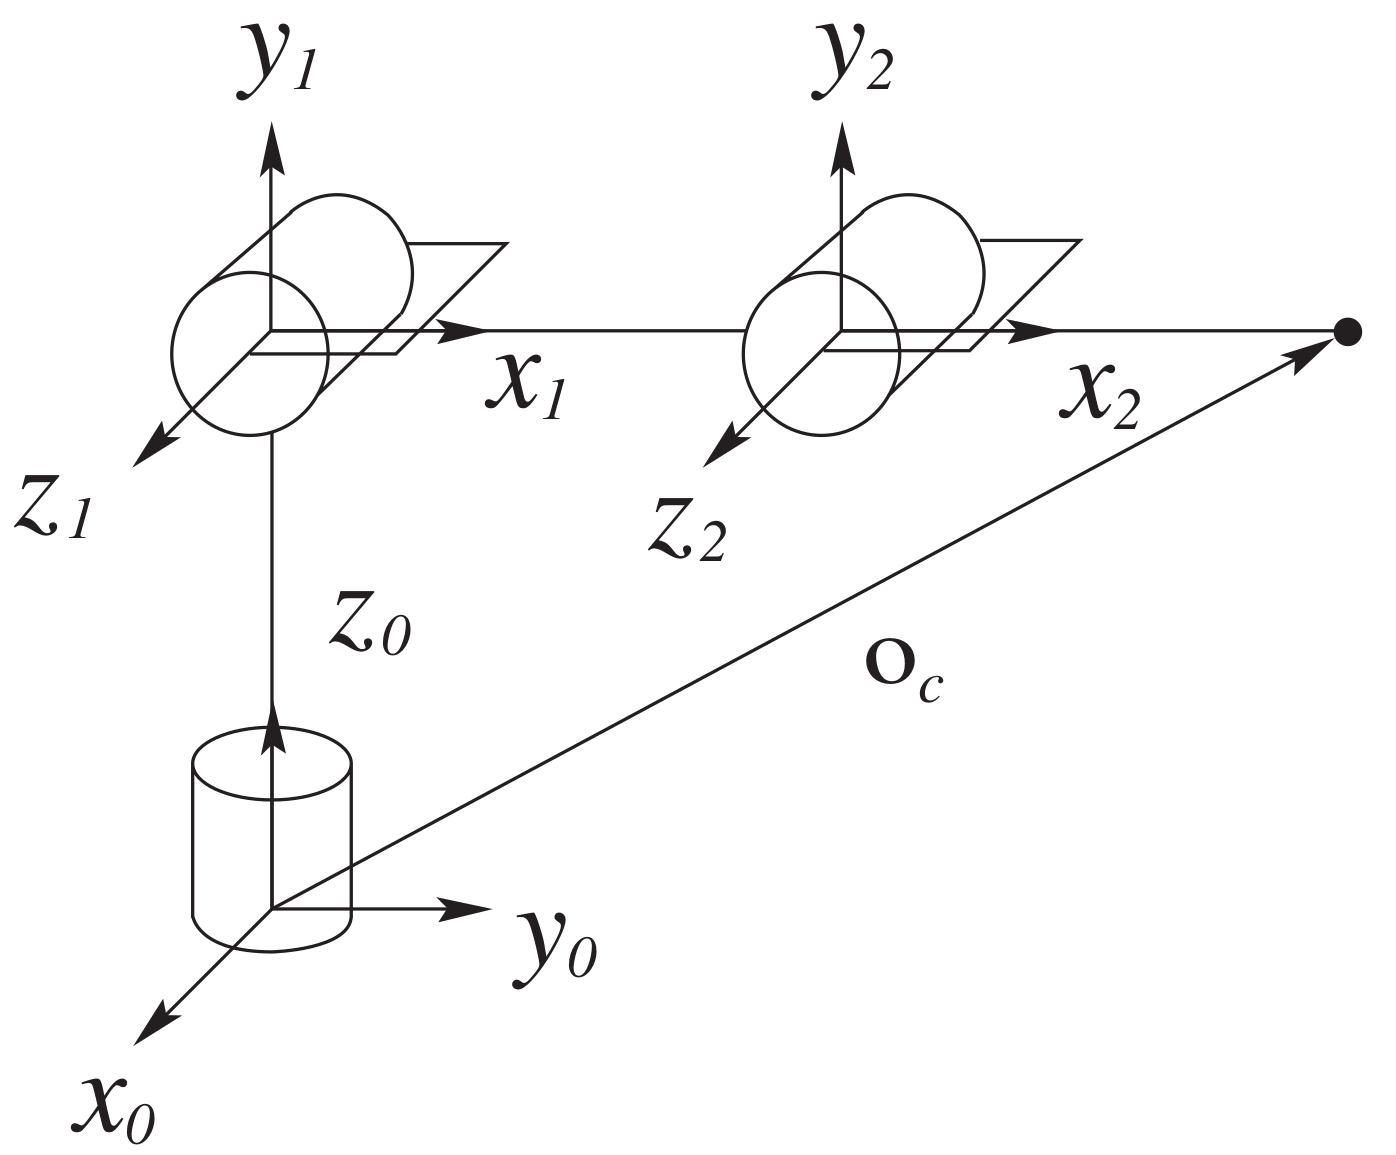
\includegraphics[width=0.85\textwidth]{figures/elbow_manipulator_sing.png} 
                % \caption{\footnotesize }
            \end{figure}
            \vspace{-2mm}
            \centering
            \footnotesize{Elbow manipulator}

            \begin{figure}[bth]
                \centering
                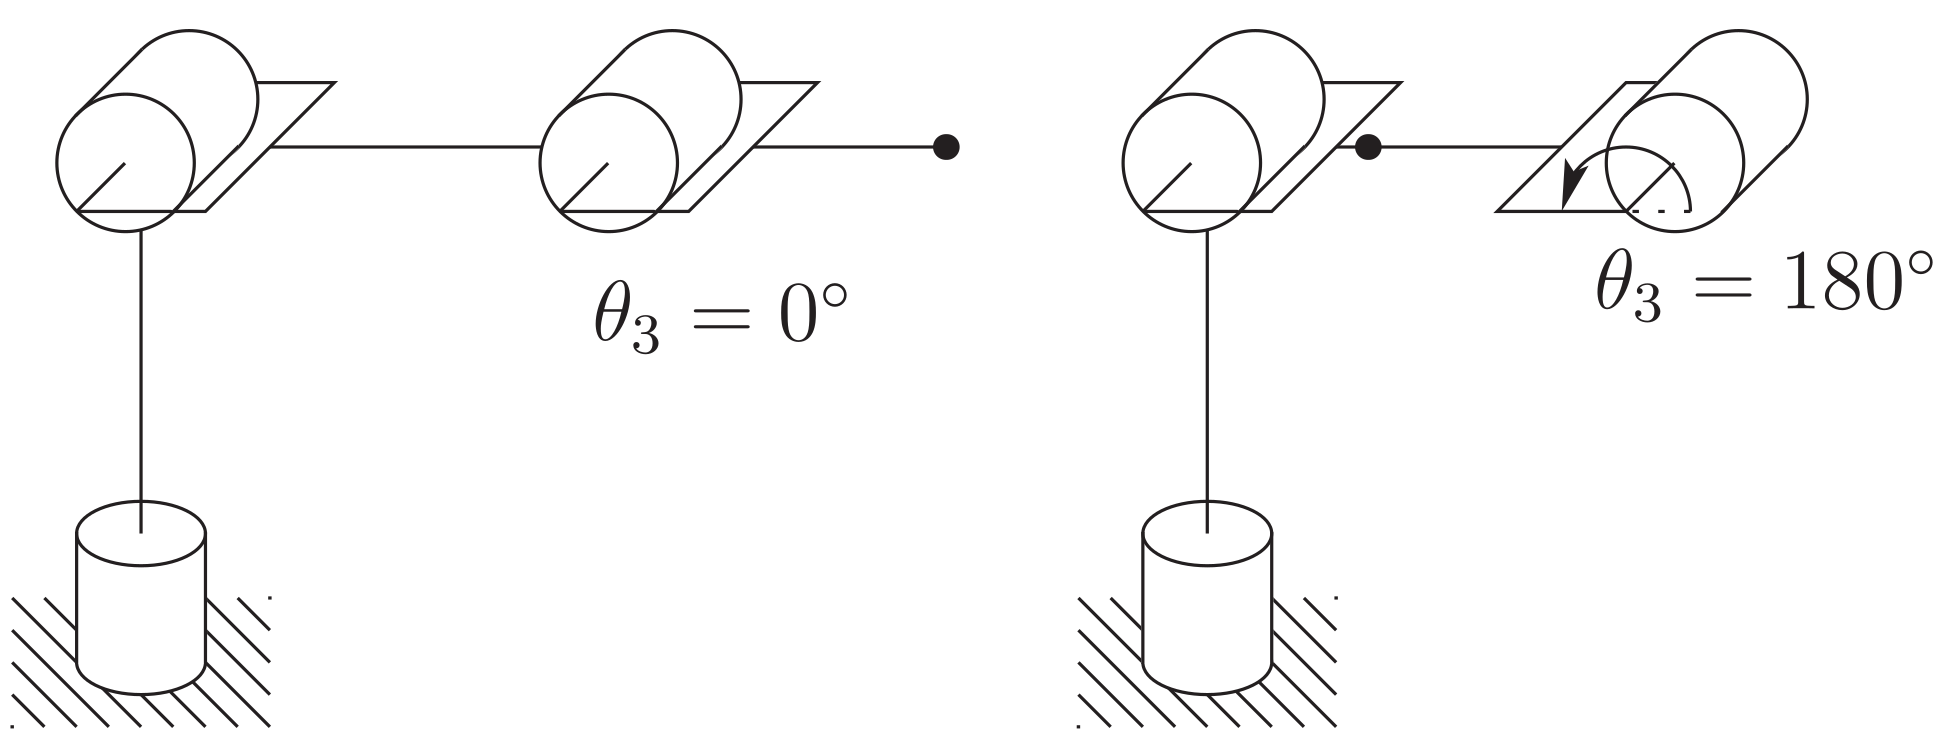
\includegraphics[width=0.85\textwidth]{figures/elbow_singularities.png} 
                % \caption{\footnotesize }
            \end{figure}
            \vspace{-2mm}
            \centering
            \footnotesize{Elbow singularities of the elbow manipulator}
        \end{column}
    \end{columns}
\end{frame}


\begin{frame}
    \frametitle{Arm Singularities of Elbow Manipulator}

    \begin{columns}
        \begin{column}{0.6\textwidth}
            \begin{itemize}
                \item The situation of 
                \[ a_2c_2 + a_3c_{23} = 0. \]
                is shown on the top right figure.
                \item This configuration occurs when the wrist center intersects
                the axis of the base rotation, $z_0$.
                \item If the elbow manipulator has an offset (bottom right
                figure), the wrist center cannot intersect $z_0$.
            \end{itemize}
        \end{column}
        \begin{column}{0.4\textwidth}
            \begin{figure}[bth]
                \centering
                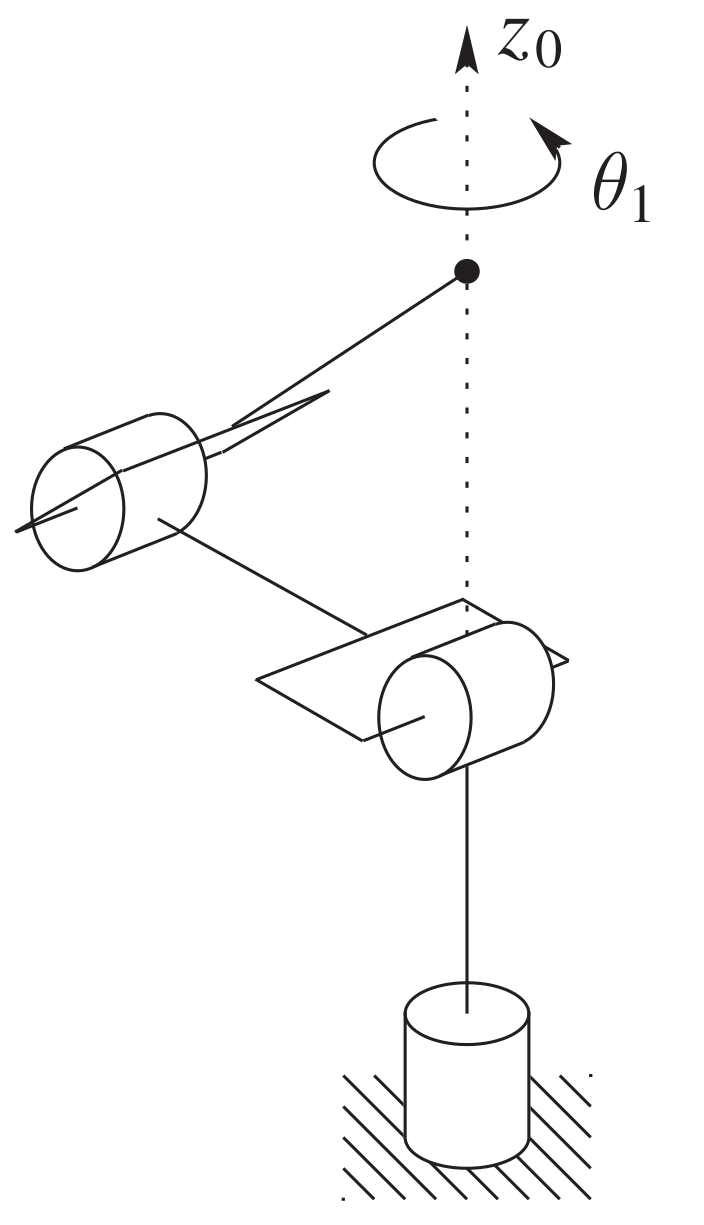
\includegraphics[width=0.4\textwidth]{figures/elbow_sing_no_offset.png} 
                % \caption{\footnotesize }
            \end{figure}
            \vspace{-2mm}
            \centering
            \footnotesize{Singularity of elbow manipulator with no offsets.}

            \begin{figure}[bth]
                \centering
                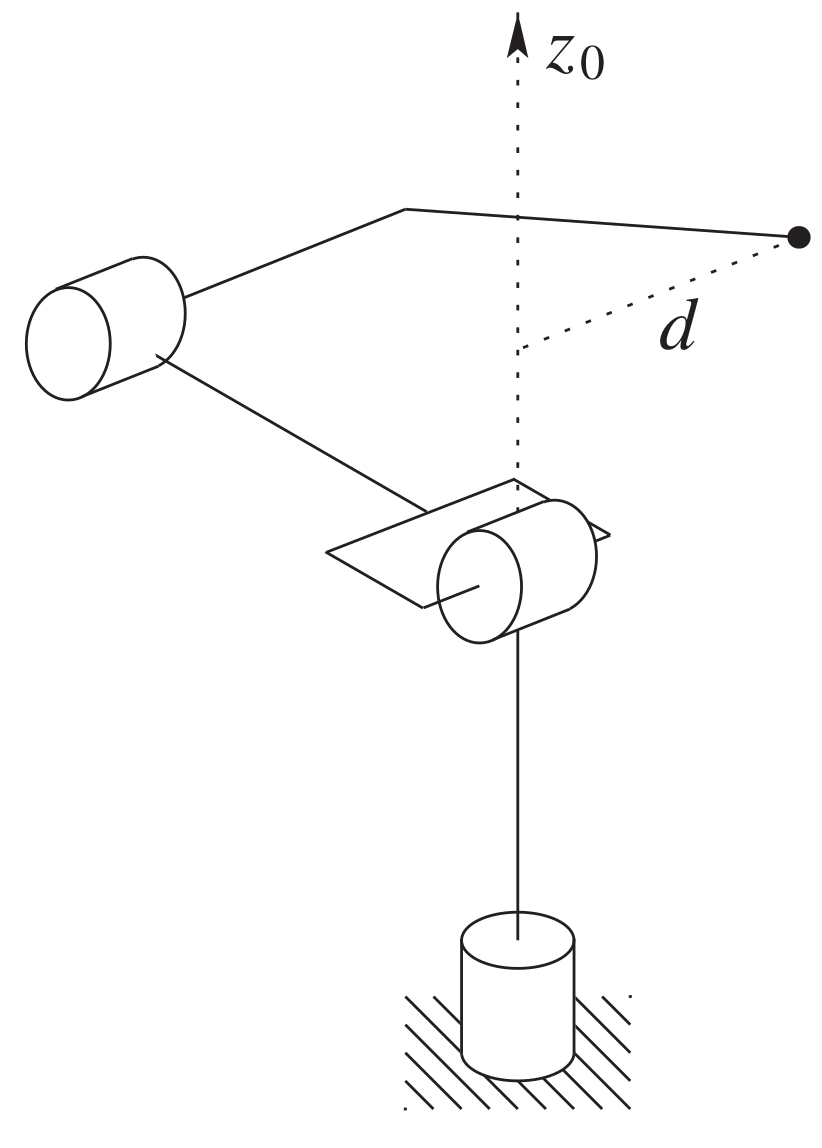
\includegraphics[width=0.4\textwidth]{figures/elbow_sing_w_offset.png} 
                % \caption{\footnotesize }
            \end{figure}
            \vspace{-2mm}
            \centering
            \footnotesize{Elbow manipulator with an offset at the elbow.}
        \end{column}
    \end{columns}
\end{frame}


\endgroup
% \section{Static Force/Torque Relationships}

\begin{frame}[standout, plain, noframenumbering]
    Static Force/Torque Relationships

    % \medskip

    % \footnotesize
    % Sam Greydanus \quad Misko Dzamba \quad Jason Yosinski
\end{frame}

\begingroup
\small


\begin{frame}
    \frametitle{Static Force/Torque Relationships}

    \begin{itemize}
        \item Interaction of the manipulator with the environment produces
        forces and moments at the end effector or tool.
        \item These produce torques at the joints of the robot.\footnotemark
        \item We discuss the role of the manipulator Jacobian in the
        quantitative relationship between the end effector forces and joint
        torques.
        \item Let $F = (F_x, F_y, F_z, n_x, n_y, n_z)$ represent the vector of 
        forces and moments at the end effector.
        \item Let $\tau$ denote the corresponding vector of joint torques. Then 
        \begin{equation}
            \boxed{\tau = J^\top(q) F.}
            \label{eq:static_force_torque}
        \end{equation} 
    \end{itemize}

    \footnotetext{We consider only revolute joints. If the joints are prismatic, 
    forces and moments at the end effector produce forces at the joints.}
\end{frame}


\begin{frame}
    \frametitle{Static Force/Torque Relationships}

    \begin{itemize}
        \item We derive the relationship~\eqref{eq:static_force_torque} through 
        the so-called \textbf{principle of virtual work}.
        \item Its detailed discussion is deferred. Instead an informal
        justification follows.
        \item Let $\delta X$ and $\delta q$ represent infinitesimal
        displacements in the task space and joint space, respectively.
        \item These displacements are called \textbf{virtual displacements} if 
        they are consistent with any constraints imposed on the system.
        \item For example, if the end effector is in contact with a rigid wall, 
        then the virtual displacements in position are tangent to the wall.
        \item These virtual displacements are related through the manipulator 
        Jacobian $J(q)$ according to 
        \begin{equation}
            \delta X = J(q) \delta q.
            \label{eq:virtual_displacement}
        \end{equation}
    \end{itemize}
\end{frame}


\begin{frame}
    \frametitle{Static Force/Torque Relationships}

    \begin{itemize}
        \item The virtual work $\delta w$ of the system is 
        \[ \delta w = F^\top \delta X - \tau^\top \delta q. \]
        \item Substituting equation~\eqref{eq:virtual_displacement} into the
        equation above yields
        \begin{equation}
            \delta w = \left( F^\top J - \tau^\top \right) \delta q.
            \label{eq:force_torque}
        \end{equation} 
        \item The principle of virtual work says that the quantity given by
        equation~\eqref{eq:force_torque} is equal to zero if the manipulator is
        in equilibrium. This gives rise to the
        equation~\eqref{eq:static_force_torque}.
    \end{itemize}
\end{frame}



\begin{frame}
    \frametitle{Example: Two-Link Planar Manipulator}

    \begin{columns}
        \begin{column}{0.6\textwidth}
            \begin{itemize}
                \item A force $F$ is applied at the end of link $2$ as shown.
                \item The Jacobian of this manipulator was formulated earlier.
                \item The resulting joint torques $\tau = (\tau_1, \tau_2)$ are 
                then given by 
            \end{itemize}
        \end{column}
        \begin{column}{0.4\textwidth}
            \begin{figure}[bth]
                \centering
                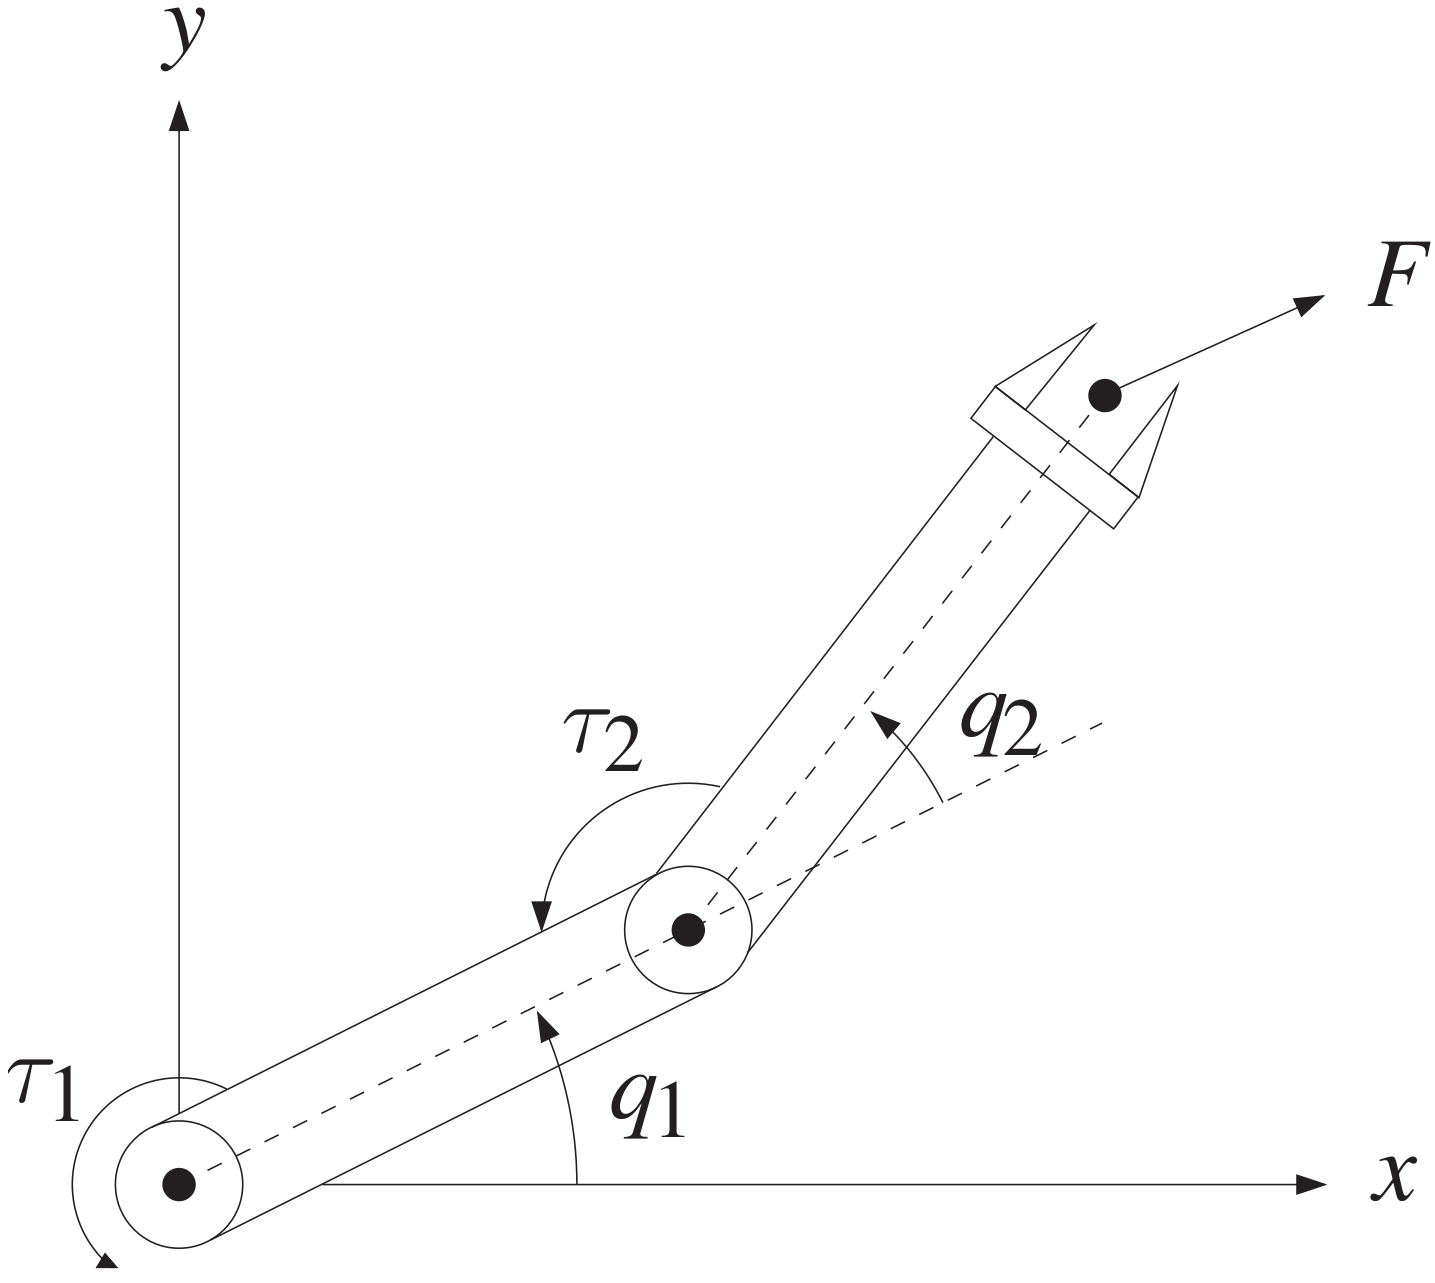
\includegraphics[width=0.85\textwidth]{figures/two_link_robot.png} 
                % \caption{\footnotesize }
            \end{figure}
            \vspace{-2mm}
            \centering
            \footnotesize{Two-link planar robot.}
        \end{column}
    \end{columns}
    \[
    \bmat{\tau_1 \\ \tau_2} = \bmat{
        -a_1s_1 - a_2s_{12} & a_1c_1 + a_2c_{12} & 0 & 0 & 0 & 1 \\ 
        -a_2s_{12} & a_2c_{12} & 0 & 0 & 0 & 1
    }\bmat{F_x \\ F_y \\ F_z \\ n_x \\ n_y \\ n_z}.
    \]
\end{frame}


\endgroup
% \section{Inverse Velocity and Acceleration}

\begin{frame}[standout, plain, noframenumbering]
    Inverse Velocity and Acceleration

    % \medskip

    % \footnotesize
    % Sam Greydanus \quad Misko Dzamba \quad Jason Yosinski
\end{frame}

\begingroup
\small


\begin{frame}
    \frametitle{Inverse Velocity and Acceleration}

    \begin{itemize}
        \item The inverse velocity problem is the problem of finding the joint
        velocities $\dot{q}$ that produce the desired end effector velocity by
        solving the equation
        \begin{equation}
            \xi = J\dot{q}
            \label{eq:vel}
        \end{equation}
        \item When the Jacobian is square and nonsingular, this problem can be 
        solved by simply inverting the Jacobian matrix, to give \[\dot{q} = J^{-1}\xi. \]
        \item For manipulators that do not have exactly six joints, the Jacobian
        cannot be inverted. In this case, there will be a solution to
        equation~\eqref{eq:vel} if and only if $\xi$ lies in the range space of
        the Jacobian. This is the case if and only if \[ \rank{J(q)} = \rank
        \hspace{-6mm} \underbrace{\bmat{J(q) | \xi}}_{\textrm{augmented matrix}}
        \hspace{-6mm}. \]
    \end{itemize}
\end{frame}


\begin{frame}
    \frametitle{Inverse Velocity and Acceleration}

    \begin{itemize}
        \item If $n > 6$, we can solve for $\dot{q}$ using the right
        pseudoinverse of $J$. Problem 4-20 shows that a solution to
        equation~\eqref{eq:vel} is given by 
        \[ \dot{q} = J^\dagger \xi + (I - J^\dagger J)b, \] in which $b \in
        \mathbb{R}^n$ is an arbitrary vector.
        \item For $m < n$, $(I - J^\dagger J) \neq 0$, and all vectors of the
        form $(I - J^\dagger J)b$ lie in the nullspace of $J$.
        \begin{itemize}
            \footnotesize{
            \item If $\dot{q}^' = (I - J^\dagger J)b$, then when the joints move 
            with velocity $\dot{q}^'$, the end effector will remain fixed since 
            $J\dot{q}^' = 0$.
            \item Thus, if $\dot{q}$ solves eqn.~\eqref{eq:vel}, then so does 
            $\dot{q} + \dot{q}^'$ with $\dot{q}^' = (I - J^\dagger J)b$, for any 
            vector $b \in \mathbb{R}^3$.
            \item If the goal is to minimize the resulting joint velocities, we 
            choose $b = 0$ (Problem 4-20).
            }
        \end{itemize}
    \end{itemize}
\end{frame}


\endgroup
% \section{Manipulability}

\begin{frame}[standout, plain, noframenumbering]
    Manipulability

    % \medskip

    % \footnotesize
    % Sam Greydanus \quad Misko Dzamba \quad Jason Yosinski
\end{frame}

\begingroup
\small


\begin{frame}
    \frametitle{Manipulability}

    \begin{itemize}
        \item For a specific configuration $q$, the Jacobian relationship
        defines the linear system given by $\xi = J\dot{q}$.
        \item We can think of $J$ as scaling the input $\dot{q}$ to produce the 
        output $\xi$.
        \item We want to characterize the output in terms of an input that has
        unit norm. Consider the set of all robot joint velocities $\dot{q}$ s.t.
        \[ \norm{\dot{q}}{}^2 = \dot{q}_1^2 + \dot{q}_2^2 + \cdots + \dot{q}_n^2 \leq 1. \]
        \item If we use the minimum norm solution $\dot{q} = J^\dagger \xi$, we
        obtain 
        \begin{equation}
            \norm{\dot{q}}{}^2 = \dot{q}^\top \dot{q} = \left( J^\dagger
        \xi \right)^\top J^\dagger \xi = \xi^\top \left( JJ^\top
        \right)^{-1}\xi.
        \label{eq:jac_scaling}
        \end{equation} 
        \item Equation~\eqref{eq:jac_scaling} gives us a quantitative
        characterization of the scaling effected by the Jacobian.
        \item If $\rank J = m$, then eqn.~\eqref{eq:jac_scaling} defines an
        $m$-dimensional ellipsoid that is known as the \textbf{manipulability
        ellipsoid}. 
    \end{itemize}
\end{frame}



\begin{frame}
    \frametitle{Manipulability}

    \begin{itemize}
        \item If the input (joint velocity) vector has unit norm, then the
        output (end-effector velocity) will lie within the ellipsoid given by 
        equation~\eqref{eq:jac_scaling}.
        \item Perfoming a singular value decomposition (SVD) of $J = U\Sigma
        V^\top$ we see that
        \[ \xi^\top \left(JJ^\top\right)^{-1}\xi = \left( U^\top \xi
        \right)^\top \Sigma_m^{-2}\left( U^\top \xi \right) \] in which 
        \[
        \Sigma_m^{-2} = \bmat{
            \sigma_1^{-2} & & & \\
            & \sigma_2^{-2} & & \\
            & & \ddots & \\
            & & & \sigma_m^{-2}
        },
        \] and $\sigma_1 \geq \sigma_2 \geq \cdots \geq \sigma_m \geq 0$.
    \end{itemize}
\end{frame}


\begin{frame}
    \frametitle{Manipulability}

    \begin{itemize}
        \item If we make the substitution $w = U^\top \xi$, then the equation in
        the previous slide becomes \[ w^\top \Sigma_m^{-2}w = \sum
        \frac{w_i^2}{\sigma_i^2} \geq 1, \] and it is clear that this is the
        equation for an axis-aligned ellipsoid in a new coordinate system that
        is obtained by rotation according to the orthogonal matrix $U^\top$.
        \item In the original coordinate system, the axes of the ellipsoid are
        given by the vectors $\sigma_i u_i$.
        \item The volume of the ellipsoid is given by
        \[ \textrm{volume} = K\sigma_1\sigma_2 \cdots \sigma_m, \] in which $K$
        is a constant that depends only on the dimension $m$ of the ellipsoid.
    \end{itemize}
\end{frame}

\begin{frame}
    \frametitle{Manipulability}
    
    \begin{itemize}
        \item The manipulability measure is given by \[ \mu =
        \sigma_1\sigma_2\cdots\sigma_m. \]
        \item Now, let's consider the special case when the robot is not
        redundant, that is, $J \in \mathbb{R}^{m \times m}$.
        \item Recall that the determinant of a product is equal to the product
        of the determinants, and that a matrix and its transpose have the same
        determinant. Thus, \[ \det JJ^\top = \lambda_1^2 \lambda_2^2 \cdots
        \lambda_m^2, \] in which $\lambda_1 \geq \lambda_2 \geq \cdots \geq
        \lambda_m$ are the eigenvalues of $J$. This leads to
        \[ \mu = \sqrt{\det JJ^\top} = \abs{\lambda_1 \lambda_2 \cdots \lambda_m} = \abs{\det J}. \]
    \end{itemize}
\end{frame}


\begin{frame}
    \frametitle{Manipulability ($\mu$) Properties}

    \begin{itemize}
        \item In general, $\mu = 0$ holds iff $\rank J < m$, i.e., when $J$ is
        not full rank.
        \item Suppose that there is some error in the measured velocity $\Delta
        \xi$. We can bound the corresponding error in the computed joint
        velocity $\Delta \dot{q}$ by \[ \left( \sigma_1 \right)^{-1} \leq
        \frac{\norm{\Delta \dot{q}}{}}{\norm{\Delta \xi}{}} \leq \left( \sigma_m
        \right)^{-1} \]
    \end{itemize}
\end{frame}


\begin{frame}
    \frametitle{Two-link Arm Manipulability}

    \begin{columns}
        \begin{column}{0.6\textwidth}
            \begin{itemize}
                \item The Jacobian is given by 
                \[
                J = \bmat{
                    -a_1s_1 - a_2s_{12} & -a_2s_{12} \\ 
                    a_1c_1 + a_2c_{12} & a_2c_{12}
                }
                \]
                and the manipulability is given by \[\mu = \abs{\det J} = a_1a_2\abs{s_2}.  \]
                \only<1>{
                \item Manipulability can be used to determine optimal
                configurations in which to perform certain tasks.
                \item It may be desirable to perform a task in the configuration
                for which the end effector has the maximum manipulability
                ($\theta_2 = \pm \frac{\pi}{2}$).
                }
                \onslide<2->{
                \item Manipulability can also be used to aid in the design of 
                manipulators.
                \item Suppose that we wish to design a two-link arm whose total
                link length $a_1 + a_2$ is fixed. What values should we choose for $a_1$ and $a_2$?
                }
            \end{itemize}
        \end{column}
        \begin{column}{0.4\textwidth}
            \begin{figure}[bth]
                \centering
                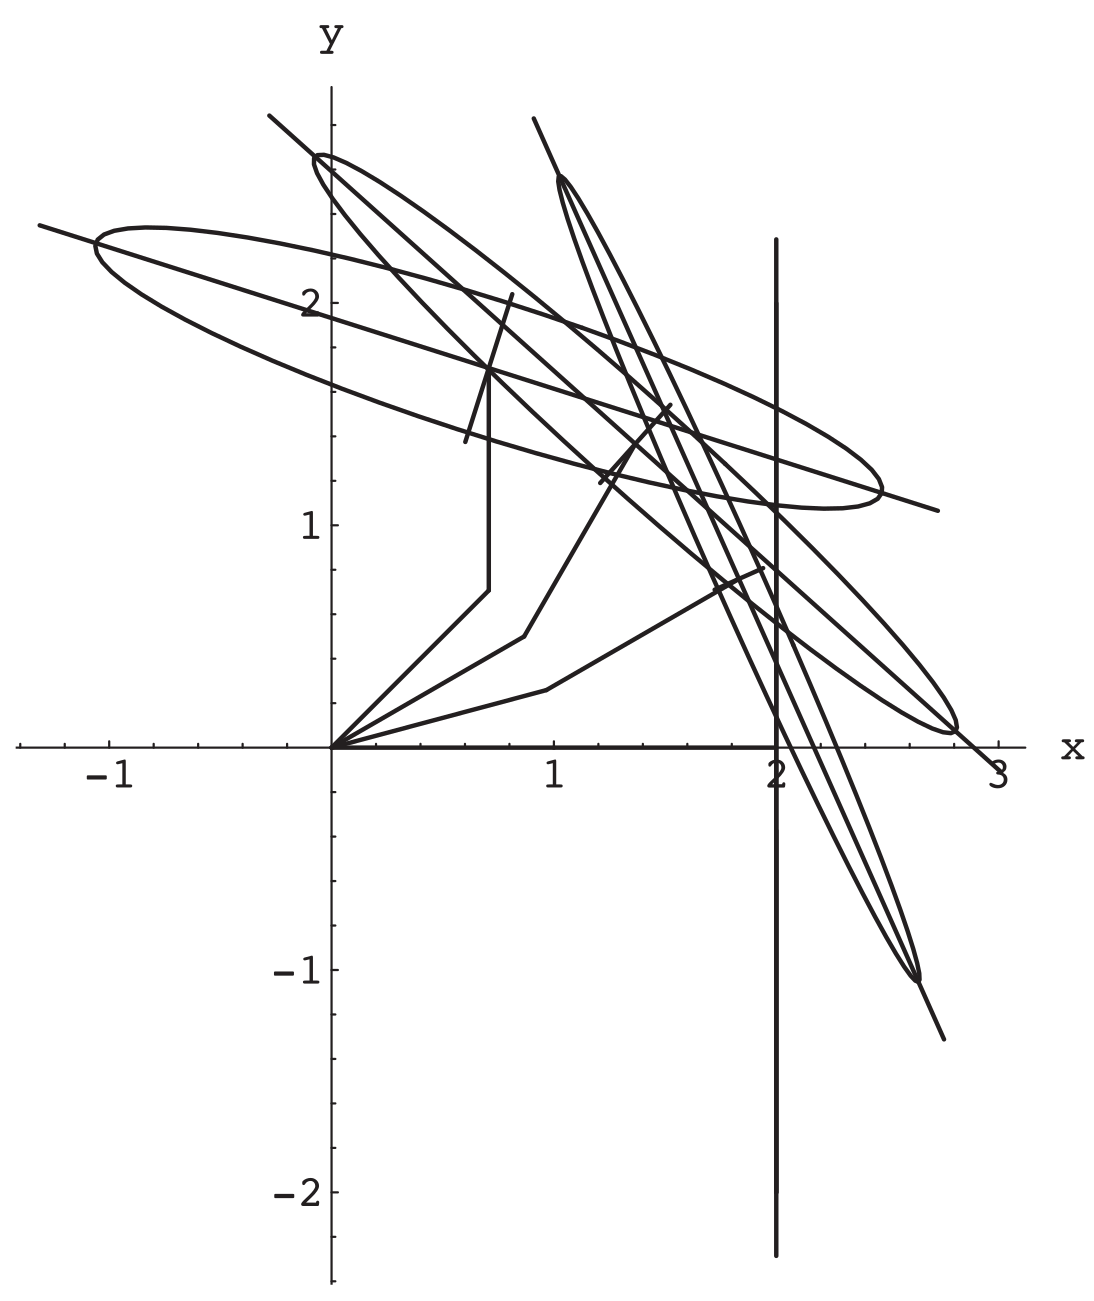
\includegraphics[width=0.85\textwidth]{figures/manipulability_ellipsoids_two_link.png} 
                % \caption{\footnotesize }
            \end{figure}
            \vspace{-2mm}
            \centering
            \footnotesize{Singularity of elbow manipulator with no offsets.}

            \vspace{3mm}
            \only<3>{
            \begin{itemize}
                \item Choose them such that the manipulability $\mu$ is maximized: $a_1 = a_2$.
            \end{itemize}
            }
        \end{column}
    \end{columns}
\end{frame}


\endgroup


%------------------------------------------------
%   The Bibliography
%------------------------------------------------
% \begin{frame}
%     \frametitle{References}
%     \bibliographystyle{abbrvnat}
%     \bibliography{wankun_thesis}
% \end{frame}

%------------------------------------------------
%   The End
%------------------------------------------------
\begin{frame}[plain, standout, noframenumbering]\end{frame}
% \appendix

\section{Similarity Transformations}

\begin{frame}[standout, plain, noframenumbering]
    Appendix

    % \medskip

    % \footnotesize
    % Sam Greydanus \quad Misko Dzamba \quad Jason Yosinski
\end{frame}

\begin{frame}
    \frametitle{Similarity Transformations -- Detailed}

    \begin{block}{Coordinate Isomorphism}
        Let $V$ be a vector space over $\mathbb{R}$ and $\mc{F} = \{f_1, \ldots,
        f_n \}$ be a basis of $V$.

        If $v \in V$, then $v = a_1f_1 + \cdots + a_n f_n$, where $a_i \in
        \mathbb{R}$ for $i = 1, \ldots, n$ are the \textit{coordinates} of $v$
        relative to $\mc{F}$. 
        
        The vector $a = \bmat{a_1 & \cdots & a_n}^\top \in
        \mathbb{R}^n$ is called the \textit{coordinate tuple} of $v$ relative to
        $\mc{F}$.

        The unique linear map $\varphi: \mathbb{R}^n \rightarrow V$ with
        $\varphi(e_j) = f_j$ for $j = 1, \ldots, n$ is called the
        \textbf{coordinate isomorphism} for $V$ and the basis $\mc{F}$. Here
        $e_j$ is the $j^{\textrm{th}}$ standard basis of $\mathbb{R}^n$.

        Thus $\varphi(a) = v$ if and only if $v = a_1 f_1 + \cdots + a_n f_n$.
    \end{block}
\end{frame}


\begin{frame}
    \frametitle{Similarity Transformations -- Detailed}

    \begin{block}{The matrix of a linear transformation}
        Let $T \in \End(V)$, i.e., $T: V \rightarrow V$ is a linear operator.
        
        The map $A = \varphi^{-1} \circ T \circ \varphi \in \End \mathbb{R}^n$
        and therefore has a matrix $[A]$; its $j^{\textrm{th}}$ column is
        $\varphi^{-1}(T(f_j))$ for $j = 1, \ldots, n$. This matrix is called the
        matrix of $T$ w.r.t. the basis $\mc{F}$.

        If $V \ni \tilde{v} = T(v)$ and $b$ and $a$ are the coordinate tuples of 
        $\tilde{v}$ and $v$, then $b = \varphi^{-1}\left(T(\varphi(a))\right) = 
        [A]a$. 

        Conversely, if $v \in V$ and $a = \varphi^{-1}(v)$ is the coordinate
        tuple of $v$ w.r.t. $\mc{F}$, and we set $b = [A]a$ and $\tilde{v} =
        \varphi(b)$, then $\tilde{v} = \varphi(A(a)) = T(v)$. That is $b = [A]a$ 
        if and only if $\tilde{v} = T(v)$.
    \end{block}
    
\end{frame}

\begin{frame}
    \frametitle{Similarity Transformations -- Detailed}

    \begin{block}{Theorem 1: Composition of linear transformations}
        Suppose $U$, $V$, and $W$ are vector spaces of finite dimension and a
        basis is chosen for each. 
        
        If $T \in \Hom(U, V)$ and $S \in Hom(V, W)$ with matrices $[A]$ and
        $[B]$, then the matrix of the linear transformation $S \circ T \in
        \Hom(U, W)$ w.r.t. the given bases is $[A][B]$.
    \end{block}
\end{frame}


\begin{frame}
    \frametitle{Similarity Transformations -- Detailed}

    Let $\mc{F} = \{f_1, \ldots, f_n \}$ and $\mc{F}^' = \{f_1^', \ldots,
    f_n^'\}$ be two bases for $V$. Let $\varphi$ and $\varphi^'$ be the
    coordinate isomorphisms, taking the standard basis in $\mathbb{R}^n$ to the
    first and second bases for $V$.

    Let $A = \varphi^{-1} \circ T \circ \varphi$, $B =
    {\left(\varphi^'\right)}^{-1} \circ T \circ {\varphi^'}$, $P = \varphi^{-1}
    \circ \varphi^'$ and $[P]$ be the matrix of $P: \mathbb{R}^n \rightarrow
    \mathbb{R}^n$. This means that element $(k,j)$, $p_{kj}$, of $[P]$ is found
    from 
    \vspace{-2mm}
    \small{
    \[ \varphi^{-1} \circ \varphi^' (e_j)  = \varphi^{-1}(f_j^') = 
     \varphi^{-1} \left( \sum_{k=1}^n p_{kj}f_k \right) = \sum_{k=1}^n p_{kj}e_k. \]}

    \vspace{-1mm}
    Similarly, the matrices $[A]$ and $[B]$ of $A$ and $B$ are found from 
    \footnotesize{
    \begin{align*}
        Ae_j &= \left( \varphi^{-1} \circ T \circ \varphi \right)e_j = 
        \varphi^{-1}\left( T(f_j) \right) = \varphi^{-1}\left( \sum_{k=1}^n 
        a_{ki}f_k \right) = \sum_{k=1}^n a_{ki} e_k. \\
        Be_j &= \left( \left(\varphi^'\right)^{-1} \circ T \circ \varphi \right)e_j = 
        \left( \varphi^'\right)^{-1}\left( T(f_j) \right) = 
        \left(\varphi^'\right)^{-1}\left( \sum_{k=1}^n b_{kj}f_k \right) = \sum_{k=1}^n b_{kj} e_k.
    \end{align*} 
    }
\end{frame}


\begin{frame}
    \frametitle{Similarity Transformations -- Detailed}

    We have
    \[ B = \left( \varphi^' \right)^{-1} \circ T \circ \varphi = \left(\varphi^'
    \right)^{-1} \circ \left(\varphi \circ A \circ \varphi^{-1}\right) \circ
    \varphi^' = P^{-1} \circ A \circ P. \]

    Now, Theorem 1 applies to yield \[ [B] = [P]^{-1} [A] [P], \] as desired.
    \hfill $\blacksquare$
\end{frame}


\begin{frame}
    \frametitle{Example 2.4 -- Revisited}

    \begin{table}
        \begin{tabular}{|c|c|c|}
            $V$ & $\mc{F}$ & $\mc{F}^'$ \\
            \hline
            $\mathbb{R}^3$ & $\left\{ x_0, y_0, z_0 \right\}$ & $\left\{ x_1,
            y_1, z_1 \right\}$
        \end{tabular}
    \end{table}

    Notice that, since $[P] = R_1^0$, we have \[ f_1^' = -f_3, \; \; f_2^' =
    f_2, \;\; f_3^' = f_1, \] i.e., \[ p_{31} = -1, \;\; p_{22} = 1, \;\; p_{13}
    = 1, \] and  
    $p_{ij} = 0$ for all other $i, j$. Furthermore, since $ A = \varphi^{-1}
    \circ T \circ \varphi$,

    \begin{table}
        \begin{tabular}{|c|c|c|c|}
            $\varphi$ & $\varphi^'$ & $\varphi^{-1} \circ \varphi^'$ & $[A]$ \\
            \hline
            $\id_{\mathbb{R}^3}$ & $P$ & $P$ & $R_{z,\theta}$
        \end{tabular}
    \end{table}

\end{frame}


\begin{frame}
    \frametitle{Example 2.4 -- Revisited}

    Let $v = 1 y_0 + 1 z_0 = -1 x_1 + y_1$. We compute,

    \vspace{-5mm}
    \[ A(v) = R_{z,\theta} \bmat{0 \\ 1 \\ 1} = \bmat{-s_\theta \\ c_\theta \\ 1}, \]
    \[
        B(v) = [P]^{-1}R_{z,\theta}[P] \bmat{-1 \\ 1 \\ 0} = 
        [P]^{-1}R_{z,\theta}\bmat{0 \\ 1 \\ 1} = [P]^{-1}\bmat{-s_\theta \\ c_\theta \\ 1} 
        = \bmat{-1 \\ c_\theta \\ -s_\theta}.
    \]

    \vspace{-5mm}
    \begin{figure}[bth]
        \centering
        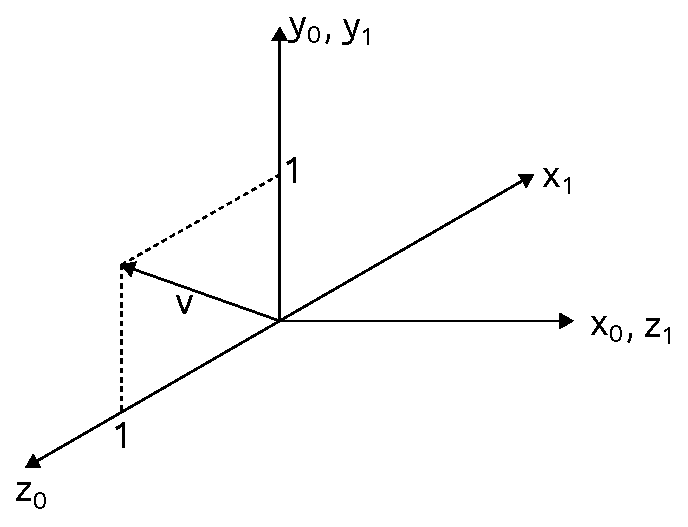
\includegraphics[width=0.5\textwidth]{figures/similarity_transform.eps}
        % \caption{\footnotesize }
    \end{figure}

\end{frame}

\begin{frame}
    \frametitle{Example 2.4 -- Revisited}

    Furthermore,
    \begin{align*}
      [B] = [P]^{-1}[A][P] &= \bmat{0 & 0 & -1 \\ 0 & 1 & 0 \\ 1 & 0 & 0}
      \bmat{c_\theta & -s_\theta & 0 \\ s_\theta & c_\theta & 0 \\ 0 & 0 & 1}
      \bmat{0 & 0 & 1 \\ 0 & 1 & 0 \\ -1 & 0 & 0} \\ &= 
      \bmat{1 & 0 & 0 \\ 0 & c_\theta & s_\theta \\ 0 & -s_\theta & c_\theta} = 
      R_{-x, \theta}.
    \end{align*}
\end{frame}

\end{document}
